\documentclass[12pt,a4paper]{article}

% --- Persian/RTL Support (XePersian) ---
% hyperref must be loaded before xepersian/bidi
\usepackage{hyperref}
\usepackage{xepersian}
\settextfont{Vazirmatn}[Scale=1.1]
\setdigitfont{Vazirmatn}[Scale=1.1]
\setlatintextfont{Libertinus Serif}
\setmonofont{Vazirmatn}

% \foreignlanguage was provided by polyglossia; keep it working via \lr
\renewcommand{\foreignlanguage}[2]{\lr{#1}}

% --- Page Layout ---
\usepackage[a4paper, top=2.5cm, bottom=2.5cm, left=2.5cm, right=2.5cm, headheight=15pt]{geometry}
\usepackage{setspace}
\onehalfspacing
\usepackage{titlesec}
\usepackage{fancyhdr}
\usepackage{lastpage}
\usepackage{xcolor}
\hypersetup{
  colorlinks=true,
  linkcolor=blue,
  citecolor=blue,
  urlcolor=blue,
  pdftitle={امنیت و حفاظت در شبکه اقتضایی خودرویی},
  pdfauthor={سید علی موسوی},
  bookmarks=true,
  bookmarksnumbered=true,
  bookmarksopen=true,
}

% --- Headers and Footers ---
\pagestyle{fancy}
\fancyhf{}
\fancyhead[L]{\small\leftmark}
\fancyhead[R]{\small حریم خصوصی و امنیت در شبکه اقتضایی خودرویی}
\fancyfoot[C]{\small صفحه \thepage\ از \pageref{LastPage}}
\renewcommand{\headrulewidth}{0.4pt}
\renewcommand{\footrulewidth}{0.4pt}

% --- Section Formatting ---
\titleformat{\section}{\Large\bfseries}{\thesection}{1em}{}
\titleformat{\subsection}{\large\bfseries}{\thesubsection}{1em}{}
\titleformat{\subsubsection}{\normalsize\bfseries}{\thesubsubsection}{1em}{}

% --- Math Packages ---
\usepackage{amsmath}
\usepackage{amssymb}
\usepackage{tikz}

% --- Table and Figure Packages ---
\usepackage{booktabs}
\usepackage{tabularx}
\usepackage{graphicx}
\usepackage{float}
\usepackage{caption}
\captionsetup{font=small, labelfont=bf}

% --- Lists ---
\usepackage{enumitem}
\setlist[itemize]{noitemsep, topsep=0pt}

% --- Line Spacing ---
\usepackage{leading}
\leading{18pt}

% --- Graphics Path ---
\graphicspath{{images/}}

% --- Bibliography ---
\usepackage[
    backend=biber,
    style=ieee,
    sorting=none
]{biblatex}

\addbibresource{report.bib}

% English, left-aligned bibliography numbers
\DeclareFieldFormat{labelnumberwidth}{\makebox[2em][l]{\lr{[#1]}}}

% --- Footnotes ---
\makeatletter
\renewcommand{\footnoterule}{%
  \kern-3pt
  \hrule width \textwidth
  \kern 2.6pt
}
\makeatother

% Paragraph formatting
\setlength{\parindent}{0pt}
\setlength{\parskip}{6pt}

% --- Title Page Info ---
\title{
  \vspace{-1cm}
  {\Huge\bfseries حریم خصوصی و امنیت در شبکه اقتضایی خودرویی} \\
}

\author{
  \vspace{1cm}
  {\large دانشکده مهندسی کامپیوتر} \\
  \vspace{1cm}
  {\large دانشجو: سید علی موسوی} \\
  \vspace{0.5cm}
  {\large استاد راهنما: دکتر بابک صادقیان} \\
  \vspace{0.5cm}
  {\large استاد درس سمینار: دکتر رضا صفابخش}
}

\date{\vspace{1cm}مردادماه ۱۴۰۵}

\begin{document}

% --- Persian Title ---
\begin{titlepage}
\begin{center}
\vspace*{0.5cm}

% University Logo

\includegraphics[width=3cm]{images/amirkabir_logo-1.png}

\vspace{0.5cm}

{\Large\textbf{دانشگاه صنعتی امیرکبیر (پلی‌تکنیک تهران)}} \\[0.3cm]
{\large\textbf{دانشکده مهندسی کامپیوتر}} \\[1.5cm]

{\Huge\textbf{حریم خصوصی و امنیت در شبکه اقتضایی خودرویی}} \\[1.5cm]

{\large\textbf{گزارش سمینار کارشناسی ارشد}} \\[1cm]

\begin{tabular}{rl}
\textbf{دانشجو:} & سید علی موسوی \\[0.3cm]
\textbf{استاد راهنما:} & دکتر بابک صادقیان \\[0.3cm]
\textbf{استاد درس سمینار:} & دکتر رضا صفابخش \\
\end{tabular}

\vspace{1.5cm}
{\large مردادماه ۱۴۰۵}

\end{center}
\end{titlepage}

% --- Abstract ---
\newpage
\begin{abstract}
شبکه‌ی اقتضایی خودرویی \LTRfootnote{\lr{Vehicular Ad-hoc Networks (VANET)}} به عنوان بخشی از سیستم‌های حمل‌ونقل هوشمند، با امکان تبادل اطلاعات بین خودروها و زیرساخت‌های جاده‌ای، نقش بسیار مهمی در بهبود ایمنی ترافیک و کاهش تصادفات ایفا می‌کنند. با این حال، ماهیت بی‌سیم و باز این شبکه‌ها، آن‌ها را در برابر حملات امنیتی مختلف مانند حملات جعل پیام، حملات سیبل، حملات فردی در میان و نقض حریم خصوصی آسیب‌پذیر می‌سازد. در این گزارش، ابتدا معماری و ویژگی‌های شبکه‌ی اقتضایی خودرویی مورد بررسی قرار می‌گیرد و سپس چالش‌های امنیتی موجود در این شبکه‌ها تحلیل می‌شود. فناوری زنجیره بلوکی به عنوان یک راهکار غیرمتمرکز برای حل مشکلات اعتماد و امنیت در شبکه‌ی اقتضایی خودرویی معرفی شده و محدودیت‌های آن در این حوزه بررسی می‌شود. \lr{IOTA Tangle} به عنوان جایگزینی مقیاس‌پذیر و بدون کارمزد برای زنجیره بلوک‌های سنتی مورد بحث قرار می‌گیرد. در نهایت، مفاهیم مدیریت هویت، شبه‌نام، هویت خودمختار \LTRfootnote{\lr{Self-Sovereign Identity (SSI)}} و شناسه‌های غیرمتمرکز \LTRfootnote{\lr{Decentralized Identifiers (DID)}} به عنوان راهکارهای نوین برای حل مشکلات امنیتی و حفظ حریم خصوصی در شبکه‌ی اقتضایی خودرویی ارائه می‌شوند. همچنین نقش روش‌های هوش مصنوعی در تقویت امنیت شبکه اقتضایی خودرویی مورد توجه ویژه قرار گرفته است.
\end{abstract}

\newpage

\tableofcontents
\newpage

% ========================================================================
% فصل ۱: مقدمه
% ========================================================================
\section{مقدمه}

در سال‌های اخیر، توسعه فناوری‌های ارتباطی و گسترش سامانه‌های حمل‌ونقل هوشمند، زمینه را برای ایجاد نسل جدیدی از وسایل نقلیه متصل و خودران فراهم کرده است. در این میان، شبکه‌ی اقتضایی خودرویی \LTRfootnote{\lr{Vehicular Ad-hoc Networks (VANET)}} به عنوان یکی از اجزای مهم سامانه‌های حمل‌ونقل هوشمند \LTRfootnote{\lr{Intelligent Transportation Systems (ITS)}}، امکان برقراری ارتباط مستقیم میان خودروها، زیرساخت‌های جاده‌ای و سایر موجودیت‌های مرتبط با محیط حمل‌ونقل را فراهم می‌کنند. هدف اصلی از ایجاد چنین شبکه‌هایی، فراهم‌کردن بستری برای تبادل سریع و قابل اعتماد اطلاعات است؛ اطلاعاتی که می‌تواند برای افزایش ایمنی، مدیریت ترافیک، ارائه خدمات هوشمند و پشتیبانی از تصمیم‌گیری خودروها مورد استفاده قرار گیرد \cite{hozouriOverviewVANETVehicular2023}.

اهمیت این فناوری را می‌توان از منظر ایمنی جاده‌ای نیز بررسی کرد. بر اساس گزارش سازمان بهداشت جهانی، سالانه بیش از ۱.۱۹ میلیون نفر در سراسر جهان بر اثر تصادفات جاده‌ای جان خود را از دست می‌دهند و تصادفات جاده‌ای یکی از مهم‌ترین عوامل مرگ‌ومیر در میان کودکان و جوانان ۵ تا ۲۹ ساله محسوب می‌شود \cite{farsimadanReviewSecurityChallenges2025}. از سوی دیگر، بخش قابل توجهی از تصادفات به خطاهای انسانی مرتبط است و در منابع مورد بررسی، بیش از ۹۲ درصد تصادفات به نوعی با خطای انسانی مرتبط دانسته شده‌اند \cite{hozouriOverviewVANETVehicular2023}. در چنین شرایطی، توانایی خودروها برای دریافت و ارسال اطلاعات مربوط به وضعیت جاده، موقعیت خودروهای اطراف، شرایط ترافیکی و رویدادهای خطرناک می‌تواند نقش مهمی در کاهش زمان واکنش راننده و افزایش ایمنی داشته باشد.

یکی از مهم‌ترین قابلیت‌های شبکه اقتضایی خودرویی، امکان انتشار هشدارهای ایمنی در زمان نزدیک به وقوع رویداد است. برای مثال، خودرو می‌تواند اطلاعات مربوط به ترمز ناگهانی، تصادف، وجود مانع در مسیر، شرایط نامناسب جاده یا تغییرات ناگهانی جریان ترافیک را به خودروهای مجاور منتقل کند. این قابلیت موجب می‌شود خودروهای حاضر در یک محدوده، تنها بر اطلاعات حاصل از حسگرهای داخلی خود متکی نباشند و بتوانند از اطلاعات تولیدشده توسط سایر خودروها و زیرساخت‌های جاده‌ای نیز استفاده کنند. در نتیجه، شبکه خودرویی می‌تواند به عنوان یک لایه ارتباطی مکمل برای سامانه‌های ایمنی و کمک‌راننده عمل کرده و زمینه را برای توسعه کاربردهای پیشرفته‌تر مانند رانندگی خودکار فراهم سازد \cite{hozouriOverviewVANETVehicular2023,xuInternetVehiclesBig2018}.

ارتباطات در این محیط محدود به ارتباط مستقیم میان دو خودرو نیست. معماری شبکه اقتضایی خودرویی می‌تواند شامل ارتباط خودرو با خودرو \LTRfootnote{\lr{Vehicle-to-Vehicle (V2V)}}، ارتباط خودرو با زیرساخت \LTRfootnote{\lr{Vehicle-to-Infrastructure (V2I)}}، ارتباط خودرو با عابر پیاده \LTRfootnote{\lr{Vehicle-to-Pedestrian (V2P)}}، ارتباط خودرو با ابر \LTRfootnote{\lr{Vehicle-to-Cloud (V2C)}} و ارتباط خودرو با شبکه‌های ارتباطی \LTRfootnote{\lr{Vehicle-to-Network (V2N)}} باشد. ترکیب این ارتباطات، محیطی را ایجاد می‌کند که در آن حجم قابل توجهی از اطلاعات میان خودروها، واحدهای کنارجاده‌ای \LTRfootnote{\lr{Road-Side Unit (RSU)}}، سامانه‌های ابری و سایر اجزای زیرساخت حمل‌ونقل مبادله می‌شود. همین افزایش سطح ارتباط، اگرچه قابلیت‌های جدیدی ایجاد می‌کند، معرض حمله و نیازمندی‌های امنیتی سامانه را نیز افزایش می‌دهد \cite{hozouriOverviewVANETVehicular2023}.

در واقع، ماهیت شبکه اقتضایی خودرویی تفاوت قابل توجهی با بسیاری از شبکه‌های سنتی دارد. خودروها گره‌هایی با تحرک بالا هستند و موقعیت آن‌ها در مدت زمان کوتاهی تغییر می‌کند. در نتیجه، توپولوژی شبکه به صورت مداوم تغییر کرده و ارتباط میان گره‌ها ممکن است به سرعت برقرار یا قطع شود. علاوه بر این، پیام‌های ایمنی معمولاً باید با تأخیر بسیار کم منتقل و پردازش شوند؛ زیرا ارزش اطلاعاتی یک پیام هشدار در بسیاری از کاربردها به زمان دریافت آن وابسته است. از سوی دیگر، تعداد زیاد خودروهای حاضر در یک محیط شهری یا بزرگراهی می‌تواند موجب افزایش شدید تعداد پیام‌ها و ایجاد ازدحام در کانال ارتباطی شود \cite{hozouriOverviewVANETVehicular2023,xuInternetVehiclesBig2018}.

این ویژگی‌ها سبب می‌شوند که تأمین امنیت در شبکه اقتضایی خودرویی صرفاً به استفاده از یک الگوریتم رمزنگاری یا یک سازوکار تصدیق هویت محدود نشود. یک سامانه امنیتی مناسب باید بتواند به صورت هم‌زمان محرمانگی، یکپارچگی، تصدیق هویت، دسترس‌پذیری، عدم انکار و حریم خصوصی را تأمین کند. از این میان، برخی الزامات ممکن است در ظاهر با یکدیگر در تضاد باشند. برای نمونه، از یک طرف لازم است فرستنده یک پیام ایمنی معتبر قابل شناسایی باشد تا خودروهای دیگر بتوانند به پیام اعتماد کنند؛ از طرف دیگر، افشای دائمی هویت واقعی خودرو می‌تواند امکان ردیابی حرکات و ایجاد نمایه رفتاری از راننده را فراهم کند. بنابراین، طراحی سازوکارهای امنیتی در این محیط نیازمند ایجاد توازن میان قابلیت اعتماد، مسئولیت‌پذیری و حفظ حریم خصوصی است \cite{farsimadanReviewSecurityChallenges2025,VanetSecurityPrivacy}.

یکی از مهم‌ترین تهدیدهای این حوزه، امکان انتشار پیام‌های جعلی یا دستکاری‌شده است. مهاجم می‌تواند با جعل هویت یک خودرو یا ایجاد پیام‌های نادرست، اطلاعاتی درباره موقعیت خودرو، وضعیت ترافیک یا وقوع یک حادثه منتشر کند. چنین حملاتی در یک شبکه خودرویی صرفاً یک تهدید اطلاعاتی محسوب نمی‌شوند، بلکه می‌توانند تصمیم‌های واقعی خودروها و رانندگان را تحت تأثیر قرار دهند. حملاتی مانند جعل پیام، جعل هویت، حمله فردی در میان \LTRfootnote{\lr{Man-in-the-Middle}}، حمله بازپخش \LTRfootnote{\lr{Replay}} و دستکاری داده‌های حسگر از جمله تهدیدهایی هستند که می‌توانند صحت و اعتمادپذیری اطلاعات مبادله‌شده را کاهش دهند \cite{farsimadanReviewSecurityChallenges2025,VanetSecurityPrivacy}.

در کنار تهدیدهای مربوط به صحت و اصالت پیام‌ها، حریم خصوصی کاربران نیز یکی از چالش‌های اساسی شبکه اقتضایی خودرویی است. خودروها در جریان ارتباطات خود ممکن است اطلاعاتی درباره موقعیت جغرافیایی، مسیر حرکت، زمان تردد و الگوی رفتاری تولید یا منتقل کنند. در صورتی که این اطلاعات بتوانند به یک هویت ثابت مرتبط شوند، مهاجم می‌تواند با تحلیل داده‌های ارتباطی، مسیر حرکت یا رفتار یک خودرو را در طول زمان دنبال کند. حملات ردیابی موقعیت، پیوندپذیری \LTRfootnote{\lr{Linkability}} و نمایه‌سازی \LTRfootnote{\lr{Profiling}} از جمله تهدیدهایی هستند که ضرورت استفاده از مکانیزم‌های اختصاصی حفظ حریم خصوصی را نشان می‌دهند \cite{farsimadanReviewSecurityChallenges2025,rahmawatiagustinaSystematicLiteratureReview2025}.

برای کاهش این خطر، استفاده از شبه‌نام‌ها \LTRfootnote{\lr{Pseudonyms}} یکی از رویکردهای رایج در طراحی سامانه‌های امنیتی شبکه‌های خودرویی است. در این رویکرد، خودرو به جای استفاده دائمی از هویت واقعی خود، از شناسه‌هایی موقت استفاده می‌کند که در بازه‌های زمانی مشخص تغییر می‌کنند. هدف از این روش، دشوار‌کردن ارتباط میان پیام‌های مختلف و یک هویت ثابت است. با این حال، استفاده از شبه‌نام به تنهایی مسئله حریم خصوصی را به طور کامل حل نمی‌کند؛ زیرا مهاجم ممکن است از اطلاعات جانبی، الگوهای مکانی یا زمانی و ویژگی‌های ترافیک برای پیوند دادن شبه‌نام‌های مختلف استفاده کند. بنابراین، طراحی چرخه کامل تولید، استفاده، تغییر و ابطال شبه‌نام‌ها همچنان یکی از مسائل مهم پژوهشی محسوب می‌شود \cite{rahmawatiagustinaSystematicLiteratureReview2025,luPseudonymChangingSocial2012}.

از سوی دیگر، یکی از محدودیت‌های رویکردهای سنتی امنیتی، وابستگی قابل توجه آن‌ها به مراجع مرکزی است. در معماری‌های مبتنی بر زیرساخت کلید عمومی \LTRfootnote{\lr{Public Key Infrastructure (PKI)}}، مرجع قابل اعتماد \LTRfootnote{\lr{Trusted Authority (TA)}} نقش مهمی در صدور و مدیریت گواهی‌ها و اعتبارنامه‌ها دارد. اگرچه این معماری می‌تواند امکان تصدیق هویت و اعتبارسنجی پیام‌ها را فراهم کند، اما وابستگی به یک مرجع مرکزی می‌تواند مسئله نقطه شکست منفرد \LTRfootnote{\lr{Single Point of Failure (SPoF)}} و همچنین چالش‌های مربوط به مقیاس‌پذیری، مدیریت گواهی و ابطال سریع اعتبارنامه‌ها را ایجاد کند \cite{rahmawatiagustinaSystematicLiteratureReview2025,VanetSecurityPrivacy}.

علاوه بر این، رمزنگاری و تصدیق هویت به تنهایی نمی‌توانند تمام تهدیدهای شبکه اقتضایی خودرویی را برطرف کنند. یک گره موذی ممکن است دارای یک گواهی معتبر باشد و از نظر رمزنگاری، پیام‌های خود را به صورت کاملاً صحیح امضا کند، اما محتوای پیام‌های آن عمداً نادرست باشد. به همین دلیل، در سال‌های اخیر موضوع مدیریت اعتماد و شهرت به عنوان مکمل سازوکارهای رمزنگاری مورد توجه قرار گرفته است.
در این رویکرد، رفتار گره‌ها بررسی شده و بر اساس سابقه عملکرد، توصیه سایر گره‌ها یا تحلیل رفتار، یک امتیاز اعتماد یا شهرت برای آن‌ها محاسبه می‌شود \cite{razaBlockchainBasedReputationTrust2024,ghovanlooyghajarSBTMSScalableBlockchain2021}.

فناوری دفترکل توزیع‌شده و به ویژه زنجیره بلوکی نیز به عنوان یکی از راهکارهای مطرح برای کاهش وابستگی به مراجع مرکزی و ایجاد یک بستر قابل اعتماد مورد توجه قرار گرفته است. ویژگی‌هایی مانند توزیع‌شدگی، تغییرناپذیری و امکان ثبت قابل بررسی رویدادها می‌توانند در مدیریت اعتماد، ثبت سوابق امنیتی، مدیریت هویت و جلوگیری از دستکاری اطلاعات مفید باشند \cite{razaBlockchainBasedReputationTrust2024,fengBPASBlockchainAssistedPrivacyPreserving2020}. با این حال، استفاده مستقیم از زنجیره بلوک‌های سنتی در محیط‌های خودرویی با محدودیت‌هایی مانند تأخیر تأیید، مقیاس‌پذیری، هزینه تراکنش و مصرف انرژی مواجه است. این محدودیت‌ها اهمیت بررسی ساختارهای جایگزین و سبک‌تر را افزایش داده‌اند.

در این زمینه، \lr{IOTA Tangle} به عنوان یک دفترکل توزیع‌شده مبتنی بر گراف جهت‌دار غیرمدور \LTRfootnote{\lr{Directed Acyclic Graph (DAG)}} مورد توجه قرار گرفته است. ساختار \lr{Tangle} با معماری متفاوت خود نسبت به زنجیره بلوکی سنتی، امکان بررسی راهکارهایی با هدف کاهش هزینه تراکنش و بهبود مقیاس‌پذیری را فراهم می‌کند. از این رو، بررسی کاربرد \lr{IOTA Tangle} در مدیریت اعتماد، اعتبارسنجی اطلاعات و مدیریت هویت در شبکه‌های خودرویی می‌تواند یکی از مسیرهای مهم پژوهشی باشد \cite{IOTATANGLE20,silvanoIotaTangleCryptocurrency2020,feraudoDIVADIDbasedReputation2024}.

هم‌زمان با توسعه این فناوری‌ها، مفاهیم جدیدتری مانند هویت خودمختار \LTRfootnote{\lr{Self-Sovereign Identity (SSI)}}، شناسه‌های غیرمتمرکز \LTRfootnote{\lr{Decentralized Identifiers (DID)}} و اعتبارنامه‌های تأییدپذیر \LTRfootnote{\lr{Verifiable Credentials (VC)}} نیز برای حل مسائل مدیریت هویت و حفظ حریم خصوصی مطرح شده‌اند. هدف این رویکردها آن است که کنترل بیشتری بر هویت دیجیتال در اختیار صاحب هویت قرار گیرد و اطلاعات هویتی تنها در حد نیاز و با کنترل مناسب افشا شود. ترکیب این مفاهیم با شبه‌نام‌ها و دفترکل‌های توزیع‌شده می‌تواند زمینه ایجاد معماری‌هایی را فراهم کند که در آن تصدیق هویت، مسئولیت‌پذیری و حفظ حریم خصوصی به صورت هم‌زمان مورد توجه قرار گیرند \cite{mazzocca2025survey,feraudoDIVADIDbasedReputation2024}.

از منظر دیگری، رشد حجم داده‌های تولیدشده توسط خودروها، پیچیدگی حملات و پویایی محیط شبکه، استفاده از روش‌های هوش مصنوعی و یادگیری ماشین را نیز به یکی از موضوعات مهم پژوهشی تبدیل کرده است. روش‌های هوشمند می‌توانند برای تشخیص ناهنجاری، شناسایی رفتارهای غیرعادی، ارزیابی اعتماد گره‌ها و تشخیص برخی حملات مورد استفاده قرار گیرند. با این حال، استفاده از هوش مصنوعی نیز بدون چالش نیست و مسائلی مانند کیفیت داده‌های آموزشی، حملات تخاصمی، مسموم‌سازی داده و حفظ حریم خصوصی باید در طراحی چنین سامانه‌هایی مورد توجه قرار گیرد \cite{farsimadanReviewSecurityChallenges2025}.

بنابراین، امنیت شبکه اقتضایی خودرویی را نمی‌توان به یک لایه یا یک فناوری خاص محدود کرد. یک معماری امنیتی جامع باید مجموعه‌ای از مکانیزم‌های رمزنگاری، تصدیق هویت، مدیریت کلید، حفظ حریم خصوصی، مدیریت اعتماد، تشخیص ناهنجاری، مدیریت هویت و در صورت نیاز فناوری‌های دفترکل توزیع‌شده را در کنار یکدیگر در نظر بگیرد. مهم‌تر از آن، این سازوکارها باید با محدودیت‌های ذاتی محیط خودرویی، از جمله تحرک بالا، تغییرات سریع توپولوژی، نیاز به تأخیر پایین، حجم بالای پیام‌ها و الزامات مقیاس‌پذیری سازگار باشند \cite{farsimadanReviewSecurityChallenges2025,rahmawatiagustinaSystematicLiteratureReview2025}.

در چنین شرایطی مسئله اصلی این گزارش بررسی معماری‌های مختلفی‌ست که به ابعاد مختلف امنیت و حریم خصوصی در شبکه اقتضایی خودرویی می‌پردازد و بررسی طرح‌هایی است که میان امنیت، حریم خصوصی، اعتماد، کارایی و مقیاس‌پذیری در شبکه‌ی اقتضایی خودرویی تعادل ایجاد کرد. این مسئله از آن جهت اهمیت دارد که افزایش امنیت نباید موجب ایجاد تأخیر غیرقابل قبول در پیام‌های ایمنی شود و حفظ حریم خصوصی نیز نباید به گونه‌ای باشد که امکان پاسخگویی در برابر رفتارهای موذی از بین برود. به بیان دیگر، هدف یک معماری مناسب آن است که خودروهای معتبر بتوانند بدون افشای غیرضروری هویت واقعی خود با یکدیگر ارتباط برقرار کنند، پیام‌های معتبر را از پیام‌های موذیانه تشخیص دهند و در صورت مشاهده رفتار غیرقانونی یا موذی، امکان شناسایی و برخورد با عامل مربوطه وجود داشته باشد \cite{rahmawatiagustinaSystematicLiteratureReview2025,VanetSecurityPrivacy}.

بر این اساس، این گزارش به بررسی جامع ابعاد مختلف امنیت و حریم خصوصی در شبکه‌ی اقتضایی خودرویی می‌پردازد. ابتدا در بخش ۲ مفهوم، معماری، اجزای اصلی و ویژگی‌های شبکه اقتضایی خودرویی معرفی می‌شود. سپس در بخش ۳ چالش‌های شبکه‌سازی، مقیاس‌پذیری و امنیتی و در بخش ۴ انواع حملات علیه این شبکه‌ها بررسی خواهند شد. سپس راهکارهای دفاعی به تفکیک بررسی می‌شوند: در بخش ۵ مکانیزم‌های حفظ حریم خصوصی شامل شبه‌نام و تکنیک‌های بی‌نامی، در بخش ۶ رمزنگاری و امضاهای دیجیتال، در بخش ۷ مدیریت اعتماد و شهرت، در بخش ۸ زنجیره بلوکی و \lr{IOTA Tangle}، در بخش ۹ مدیریت هویت با شناسه‌های غیرمتمرکز و اعتبارنامه‌های تأییدپذیر، در بخش ۱۰ نقش هوش مصنوعی در تشخیص ناهنجاری. همچنین در بخش ۱۱ فناوری‌های نوظهور مانند \lr{5G/6G}، رایانش لبه و مه، و در بخش ۱۲ لایه سخت‌افزاری به عنوان بخش پشتیبان امنیت مورد توجه قرار می‌گیرند. در نهایت،  در بخش ۱۳ مسائل باز، جهت‌گیری‌های پژوهشی آینده و در بخش ۱۴ جمع‌بندی کلی ارائه می‌شود.

% ========================================================================
% فصل ۲: شبکه اقتضایی خودرویی چیست؟
% ========================================================================
\section{شبکه اقتضایی خودرویی چیست؟}

\subsection{تعریف و مفهوم}

شبکه اقتضایی خودرویی یک زیرمجموعه از شبکه‌های خودمختار متحرک \LTRfootnote{\lr{Mobile Ad-hoc Networks (MANET)}} است که ارتباط بین خودروهای نزدیک و بین خودروها و زیرساخت‌ها را تسهیل می‌کند \cite{hozouriOverviewVANETVehicular2023}. در این شبکه‌ها، خودروها به عنوان گره‌های متحرک عمل کرده و اطلاعات ایمنی و ترافیکی را با یکدیگر به اشتراک می‌گذارند \cite{xuInternetVehiclesBig2018}. خودروهای متصل با امکان ارتباط با محیط داخلی و خارجی خود، بخشی جدایی‌ناپذیر از زندگی مدرن شده‌اند و پیش‌بینی شده بود بازار جهانی خودروهای متصل تا سال ۲۰۱۹ به ۱۳۱.۹ میلیارد دلار برسد \cite{luConnectedVehiclesSolutions2014}.

\begin{figure}[H]
\centering
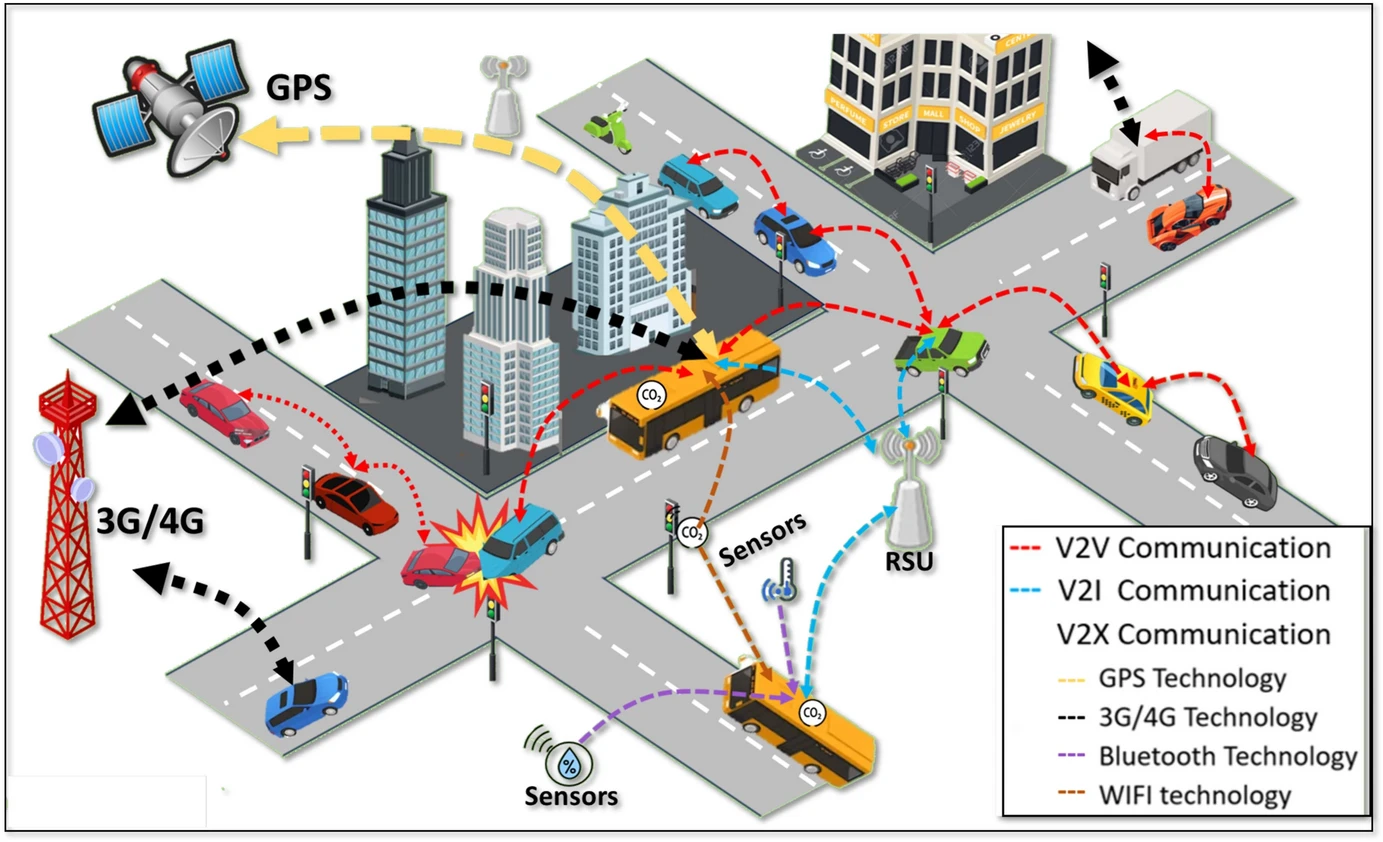
\includegraphics[width=0.9\textwidth]{VANET artitecture.png}
\caption{معماری شبکه اقتضایی خودرویی و انواع ارتباطات خودرو با هر موجودیت}
\label{fig:vanet_arch}
\end{figure}

\subsection{ارکان اصلی شبکه اقتضایی خودرویی}

ارکان اصلی شبکه اقتضایی خودرویی عبارتند از:

\begin{itemize}
  \item \textbf{واحدهای سوارشونده \LTRfootnote{\lr{On-Board Unit (OBU)}}}: سخت‌افزارهایی که در هر خودرو نصب شده و امکان ارتباط با واحدهای کنارجاده‌ای و واحدهای سوارشونده دیگر را فراهم می‌کنند \cite{hozouriOverviewVANETVehicular2023}.
  \item \textbf{واحدهای کنارجاده‌ای \LTRfootnote{\lr{Road-Side Unit (RSU)}}}: واحدهای ثابتی که در کنار جاده‌ها نصب شده و ارتباط خودروها با زیرساخت را برقرار می‌کنند \cite{hozouriOverviewVANETVehicular2023}.
  \item \textbf{مرجع قابل اعتماد \LTRfootnote{\lr{Trusted Authority (TA)}}}: مرجع مرکزی مسئول مدیریت امنیت و صدور اعتبارنامه‌ها \cite{rahmawatiagustinaSystematicLiteratureReview2025}.
\end{itemize}

\subsection{معماری و انواع ارتباطات}

شکل \ref{fig:vanet_arch} معماری کلی شبکه اقتضایی خودرویی و انواع ارتباطات خودرو با هر موجودیت \LTRfootnote{\lr{Vehicle-to-Everything (V2X)}} را نشان می‌دهد:

\begin{itemize}
  \item \textbf{ارتباط خودرو به خودرو \LTRfootnote{\lr{Vehicle-to-Vehicle (V2V)}}}: تبادل مستقیم اطلاعات بین خودروهای مجاور.
  \item \textbf{ارتباط خودرو به زیرساخت \LTRfootnote{\lr{Vehicle-to-Infrastructure (V2I)}}}: تبادل اطلاعات بین خودرو و واحدهای کنارجاده‌ای.
  \item \textbf{ارتباط خودرو به عابر پیاده \LTRfootnote{\lr{Vehicle-to-Pedestrian (V2P)}}}: هشدار به عابران پیاده مجهز به دستگاه‌های همراه.
  \item \textbf{ارتباط خودرو به ابر \LTRfootnote{\lr{Vehicle-to-Cloud (V2C)}}}: تبادل اطلاعات با سرویس‌های ابری.
  \item \textbf{ارتباط خودرو به پهپاد \LTRfootnote{\lr{Vehicle-to-UAV (VTU)}}}: بهره‌گیری از پهپادها برای اطلاعات ترافیکی و ایمنی.
  \item \textbf{ارتباط خودرو به شبکه \LTRfootnote{\lr{Vehicle-to-Network (V2N)}}}: ارتباط با شبکه‌های سلولی مانند \lr{5G}.
\end{itemize}

\subsection{اهمیت شبکه اقتضایی خودرویی}

اهمیت شبکه اقتضایی خودرویی از جنبه‌های مختلفی قابل بررسی است:

\begin{itemize}
  \item \textbf{ایمنی ترافیک:} ارائه هشدارهای ایمنی بلادرنگ مانند هشدار تصادف جلو، هشدار تغییر لاین و هشدار شرایط جاده \cite{hozouriOverviewVANETVehicular2023}.
  \item \textbf{بهینه‌سازی ترافیک:} مدیریت هوشمند تقاطع‌ها، کاهش ازدحام و بهبود جریان ترافیک \cite{xuInternetVehiclesBig2018}.
  \item \textbf{سرویس‌های اطلاعاتی:} ارائه اطلاعات ناوبری، شرایط آب‌وهوا و سرویس‌های سرگرمی \cite{hozouriOverviewVANETVehicular2023}.
  \item \textbf{خودروهای خودران:} پشتیبانی از رانندگی خودکار از طریق تبادل اطلاعات بلادرنگ \cite{xuInternetVehiclesBig2018}.
\end{itemize}

\subsection{ویژگی‌های متمایز}

شبکه اقتضایی خودرویی ویژگی‌های منحصربه‌فردی دارد که آن‌ها را از سایر شبکه‌های بی‌سیم متمایز می‌سازد \cite{hozouriOverviewVANETVehicular2023}:

\begin{itemize}
  \item \textbf{تحرک بالا:} گره‌ها می‌توانند سرعت‌های بالایی داشته باشند.
  \item \textbf{تغییرات مکرر توپولوژی:} ساختار شبکه به طور مداوم تغییر می‌کند.
  \item \textbf{محدودیت منابع پردازشی:} برخلاف فرض رایج، خودروها انرژی فراوان دارند اما واحدهای سوارشونده و واحدهای کنارجاده‌ای در پردازش و ذخیره‌سازی محدود هستند؛ از این رو استفاده از رمزنگاری سبک (مانند \lr{ECC}، \lr{IBC} و تأیید دسته‌ای) ضروری است \cite{farsimadanReviewSecurityChallenges2025}.
  \item \textbf{تأخیر کم:} ارتباطات بلادرنگ برای سرویس‌های ایمنی ضروری است.
  \item \textbf{امنیت داده‌ها:} داده‌ها باید رمزنگاری شده و از تغییر محافظت شوند.
\end{itemize}

% ========================================================================
% فصل ۳: چالش‌ها و الزامات امنیتی
% ========================================================================
\section{چالش‌های شبکه اقتضایی خودرویی}

\subsection{چالش‌های شبکه‌سازی}

شبکه اقتضایی خودرویی با چالش‌های متعددی در حوزه شبکه‌سازی مواجه است \cite{hozouriOverviewVANETVehicular2023}:

\begin{itemize}
  \item \textbf{تکه‌تکه شدن مکرر شبکه:} تراکم و تحرک بالای گره‌ها باعث قطع و وصل مکرر اتصالات می‌شود.
  \item \textbf{مشکلات مسیریابی:} یافتن مسیر مناسب برای ارسال پیام‌ها در شبکه‌های پویا دشوار است؛ این موضوع پیش‌درآمدی بر حملات لایه مسیریابی است که در فصل ۴ بررسی می‌شود.
  \item \textbf{کمبود طیف فرکانسی:} استاندارد \lr{DSRC} دارای مشکلات قابلیت اطمینان و مقیاس‌پذیری است.
  \item \textbf{تأثیرات محیطی:} ساختمان‌ها، خودروها و درختان می‌توانند سیگنال‌ها را مختل کنند.
\end{itemize}

\subsection{چالش‌های مدیریت منابع}

مدیریت منابع در شبکه اقتضایی خودرویی با چالش‌های زیر مواجه است \cite{hozouriOverviewVANETVehicular2023, niSecuringFogComputing2018}:

\begin{itemize}
  \item \textbf{منابع مشترک:} کانال‌های پهنای باند و واحدهای کنارجاده‌ای منابع مشترکی هستند که باید بهینه مدیریت شوند.
  \item \textbf{تخصیص منابع رادیویی:} تکنیک‌های کنترل دسترسی رسانه \LTRfootnote{\lr{MAC}} برای تضمین دسترسی عادلانه به کانال ضروری هستند.
  \item \textbf{هزینه استقرار:} استقرار زیرساخت شبکه اقتضایی خودرویی نیازمند سرمایه‌گذاری قابل توجهی است.
\end{itemize}

\subsection{چالش‌های مقیاس‌پذیری}

مقیاس‌پذیری یکی از مهمترین چالش‌های شبکه اقتضایی خودرویی است \cite{xuInternetVehiclesBig2018}:

\begin{itemize}
  \item افزایش تعداد خودروهای متصل نیازمند مدیریت حجم عظیمی از داده‌ها است.
  \item حجم داده‌های تولید شده توسط خودروهای هوشمند به هزاران گیگابایت در روز می‌رسد.
  \item پردازش بلادرنگ این حجم از داده‌ها نیازمند منابع محاسباتی قابل توجهی است.
\end{itemize}

\subsection{چالش‌های استانداردسازی}

عدم وجود استانداردهای یکپارچه یکی دیگر از چالش‌های مهم است \cite{farsimadanReviewSecurityChallenges2025}:

\begin{itemize}
  \item تنوع فناوری‌های ارتباطی\LTRfootnote{\lr{DSRC, LTE, 5G}} و نیاز به سازگاری بین آن‌ها.
  \item نیاز به استانداردهای مشترک برای تبادل پیام‌ها و تصدیق هویت.
  \item چالش‌های بین‌المللی در یکپارچه‌سازی سیستم‌های مختلف.
\end{itemize}

\subsection{چالش‌های امنیتی}

برای تضمین امنیت شبکه اقتضایی خودرویی، الزامات زیر باید برآورده شوند \cite{farsimadanReviewSecurityChallenges2025, VanetSecurityPrivacy}:

\begin{itemize}
\item \textbf{دسترس‌پذیری\LTRfootnote{\lr{Availability}}:} ارتباطات باید به موقع در دسترس گیرندگان مورد نظر باشند.
\item \textbf{محرمانگی\LTRfootnote{\lr{Confidentiality}}:} داده‌ها باید رمزنگاری و محافظت شوند.
\item \textbf{تصدیق هویت\LTRfootnote{\lr{Authentication}}:} تمایز بین اشیاء معتبر و عناصر موذی.
\item \textbf{یکپارچگی\LTRfootnote{\lr{Integrity}}:} داده‌ها باید به موقع تأیید شوند.
\item \textbf{عدم انکار\LTRfootnote{\lr{Non-repudiation}} و پاسخگویی\LTRfootnote{\lr{Accountability}}:} جلوگیری از انکار پیام‌ها از طریق \lr{PKI}، برچسب زمانی و ثبت امن \cite{VanetSecurityPrivacy}.
\item \textbf{حریم خصوصی\LTRfootnote{\lr{Privacy}}:} محافظت از اطلاعات شخصی کاربران.
\item \textbf{اعتماد\LTRfootnote{\lr{Trust}}:} اطمینان بین موجودیت‌ها برای انتقال امن داده‌ها.
\end{itemize}

% ========================================================================
% فصل ۴: حملات امنیتی
% ========================================================================
\section{حملات امنیتی بر روی شبکه اقتضایی خودرویی}

\subsection{الگوی تهدید}

شبکه اقتضایی خودرویی در برابر حملات امنیتی مختلفی آسیب‌پذیر است. بر اساس مطالعات انجام‌شده، تحلیل تهدیدات و معماری امنیتی شبکه اقتضایی خودرویی نشان می‌دهد که حفظ تعادل بین کاهش مؤثر تهدیدات و حداقل تأثیر بر عملکرد سیستم از اهمیت بالایی برخوردار است \cite{SecuringVehicularAd, farsimadanReviewSecurityChallenges2025, VanetSecurityPrivacy, linGSISSecurePrivacyPreserving2007}. در مدل تهدید، مهاجمان به دو دسته تقسیم می‌شوند: مهاجمان بیرونی که به شبکه دسترسی ندارند و گره‌های موذی داخلی که دارای گواهی‌های معتبر هستند اما رفتاری موذی دارند \cite{farsimadanReviewSecurityChallenges2025}.

\subsection{حملات بر دسترس‌پذیری}

\begin{itemize}
  \item \textbf{حملات ممانعت ازسرویس\LTRfootnote{\lr{DoS/DDoS}}:} اشباع واحدهای کنارجاده‌ای و شبکه با ترافیک اضافی برای جلوگیری از عملکرد صحیح \cite{farsimadanReviewSecurityChallenges2025}.
  \item \textbf{سیل پیام\LTRfootnote{\lr{Flooding}}:} طوفان پخش پیام برای اشباع پهنای باند \cite{VanetSecurityPrivacy}.
  \item \textbf{ممانعت ازسرویس مبتنی بر حافظه\LTRfootnote{\lr{Memory-based DoS}}:} تخلیه حافظه واحدهای سوارشونده و واحدهای کنارجاده‌ای \cite{rahmawatiagustinaSystematicLiteratureReview2025}.
  \item \textbf{پارازیت\LTRfootnote{\lr{Jamming}}:} اختلال در کانال‌های بی‌سیم در لایه فیزیکی \cite{farsimadanReviewSecurityChallenges2025}.
\end{itemize}

\subsection{حملات بر محرمانگی}

\begin{itemize}
  \item \textbf{استراق سمع\LTRfootnote{\lr{Eavesdropping}}:} دسترسی غیرمجاز به اطلاعات خصوصی از طریق شنود ترافیک بی‌سیم \cite{farsimadanReviewSecurityChallenges2025}.
  \item \textbf{تحلیل ترافیک\LTRfootnote{\lr{Traffic analysis}}:} استنتاج الگوهای رفتاری و مکانی از روی ترافیک مشاهده‌شده \cite{farsimadanReviewSecurityChallenges2025}.
  \item \textbf{حملات کانال جانبی\LTRfootnote{\lr{Side-channel}}:} استخراج کلیدهای رمزنگاری از طریق نشت زمان‌بندی، توان مصرفی یا تابش الکترومغناطیسی \cite{rahmawatiagustinaSystematicLiteratureReview2025}.
\end{itemize}

\subsection{حملات بر صحت، یکپارچگی و تصدیق هویت}

\begin{itemize}
  \item \textbf{جعل پیام\LTRfootnote{\lr{Spoofing/Forgery}}:} تولید اطلاعات نادرست یا جعلی \cite{farsimadanReviewSecurityChallenges2025}.
  \item \textbf{جعل هویت\LTRfootnote{\lr{Impersonation/Masquerade}}:} مهاجمان خود را به جای واحدهای سوارشونده یا واحدهای کنارجاده‌ای جا می‌زنند \cite{VanetSecurityPrivacy}.
  \item \textbf{دستکاری پیام\LTRfootnote{\lr{Message tampering}}:} تغییر، حذف یا اصلاح داده‌ها در حین انتقال \cite{farsimadanReviewSecurityChallenges2025}.
  \item \textbf{حمله پخش مجدد\LTRfootnote{\lr{Replay}}:} استفاده مجدد از پیام‌های معتبر ضبط‌شده؛ مقابله با برچسب زمانی و امضای سبک \lr{TESLA++} انجام می‌شود \cite{farsimadanReviewSecurityChallenges2025, VanetSecurityPrivacy}.
  \item \textbf{حمله فردی در میان\LTRfootnote{\lr{Man-in-the-Middle}}:} رهگیری و تغییر ارتباط بین دو طرف \cite{farsimadanReviewSecurityChallenges2025}.
  \item \textbf{حملات جعل موقعیت و داده حسگر:} جعل \lr{GPS}، خودروی پنهان\LTRfootnote{\lr{Hidden vehicle}} و حمله توهم\LTRfootnote{\lr{Illusion attack}} که با دستکاری داده حسگرها ادراک نادرست ایجاد می‌کند \cite{farsimadanReviewSecurityChallenges2025}.
  \item \textbf{حمله ربایش نشست\LTRfootnote{\lr{Session hijacking}}:} تصاحب نشست ارتباطی احرازشده \cite{farsimadanReviewSecurityChallenges2025}.
  \item \textbf{کد موذیانه\LTRfootnote{\lr{Malicious code}}:} تزریق بدافزار به گره‌های خودرو \cite{farsimadanReviewSecurityChallenges2025}.
\end{itemize}

\subsection{حملات بر حریم خصوصی}

\begin{itemize}
  \item \textbf{افشای هویت\LTRfootnote{\lr{Identity disclosure}}:} نقض اطلاعات هویتی سرنشینان خودرو \cite{farsimadanReviewSecurityChallenges2025}.
  \item \textbf{ردیابی موقعیت و مسیر\LTRfootnote{\lr{Location tracking}}:} ردیابی موقعیت و مسیر خودرو توسط مهاجم \cite{farsimadanReviewSecurityChallenges2025}.
  \item \textbf{حمله پیوندپذیری\LTRfootnote{\lr{Linkability}}:} اتصال چند شبه‌نام یا پیام به یک خودروی واحد \cite{rahmawatiagustinaSystematicLiteratureReview2025}.
  \item \textbf{نمایه‌سازی\LTRfootnote{\lr{Profiling}}:} ایجاد نمایه رفتاری و هویتی در طول زمان \cite{VanetSecurityPrivacy}.
  \item \textbf{دسترسی غیرمجاز:} دور زدن کنترل دسترسی و بهره‌برداری از شکاف ابطال گواهی \cite{rahmawatiagustinaSystematicLiteratureReview2025}.
\end{itemize}

\subsection{حملات رفتاری گره‌های داخلی}

\begin{itemize}
  \item \textbf{رفتار خودخواهانه\LTRfootnote{\lr{Selfish behavior}}:} حذف یا تغییر وظایف رله برای منافع شخصی \cite{farsimadanReviewSecurityChallenges2025}.
  \item \textbf{انکار\LTRfootnote{\lr{Repudiation}}:} انکار ارسال یا دریافت پیام‌ها؛ مقابله با عدم انکار مبتنی بر \lr{PKI} و ثبت امن \cite{VanetSecurityPrivacy}.
  \item \textbf{تبانی\LTRfootnote{\lr{Collusion}}:} تقلب هماهنگ بین چند گره برای فریب سیستم \cite{rahmawatiagustinaSystematicLiteratureReview2025}.
  \item \textbf{حمله گودال سیاه\LTRfootnote{\lr{Blackhole}}:} حذف و انداختن بسته‌های عبوری به عنوان رفتار موذی \cite{farsimadanReviewSecurityChallenges2025}.
\end{itemize}

\subsection{حملات لایه مسیریابی و شبکه}

\begin{itemize}
  \item \textbf{حملات بر پروتکل‌های مسیریابی\LTRfootnote{\lr{AODV/GPSR}}:} گودال سیاه، انداختن بسته و سیل \cite{VanetSecurityPrivacy}.
  \item \textbf{دستکاری بسته‌ها در ارسال چندپرشی\LTRfootnote{\lr{Multi-hop rebroadcast}}:} بهره‌برداری از بازپخش ناامن پیام‌های ایمنی \cite{farsimadanReviewSecurityChallenges2025}.
\end{itemize}

\subsection{حملات سخت‌افزاری، فیزیکی و فناوری‌های ارتباطی}

\begin{itemize}
  \item \textbf{دستکاری سخت‌افزار\LTRfootnote{\lr{Hardware tampering}}:} استخراج فیزیکی کلیدها و داده‌ها از تجهیزات \cite{farsimadanReviewSecurityChallenges2025}.
  \item \textbf{حملات ورود بدون کلید از راه دور\LTRfootnote{\lr{RKE}}:} پخش مجدد، شبیه‌سازی (\lr{Hitag2})، پارازیت و فردی در میان \cite{farsimadanReviewSecurityChallenges2025}.
  \item \textbf{حمله دوقلوی شیطانی\LTRfootnote{\lr{Evil Twin}}:} جعل نقطه دسترسی \lr{Wi-Fi} برای فریب خودرو \cite{farsimadanReviewSecurityChallenges2025}.
\end{itemize}

\subsection{حملات زیرساخت و اعتماد}

\begin{itemize}
  \item \textbf{نقطه شکست منفرد\LTRfootnote{\lr{SPoF}}:} در خطر افتادن مرجع قابل اعتماد\LTRfootnote{\lr{TA}} کل شبکه را به خطر می‌اندازد؛ راهکار پیشنهادی تفکیک مرجع به دو بخش ردیابی\LTRfootnote{\lr{TRA}} و تولید کلید\LTRfootnote{\lr{KGC}} است \cite{rahmawatiagustinaSystematicLiteratureReview2025}. در این معماری، \lr{KGC} مسئول تولید و توزیع کلیدهای رمزنگاری است، در حالی که \lr{TRA} وظیفه ردیابی هویت واقعی خودروها در صورت وقوع جرم یا تخلف را بر عهده دارد. این تفکیک مانع از آن می‌شود که یک نهاد واحد بتواند هم هویت کاربران را فاش کند و هم کلیدهای رمزنگاری را در اختیار داشته باشد.
  \item \textbf{مسئله مرجع حل هویت\LTRfootnote{\lr{Privacy-authority problem}}:} توانایی مرجع در ردیابی هویت واقعی در تعارض با بی‌نامماندن است \cite{rahmawatiagustinaSystematicLiteratureReview2025}.
\end{itemize}

% ========================================================================
% فصل ۵: مکانیزم‌های حفظ حریم خصوصی
% ========================================================================
\section{مکانیزم‌های حفظ حریم خصوصی}

\subsection{شبه‌نام و چرخه حیات آن}

شبه‌نام \LTRfootnote{\lr{Pseudonym}} یک شناسه موقت و غیرقابل پیوند است که به جای هویت واقعی استفاده می‌شود \cite{rahmawatiagustinaSystematicLiteratureReview2025, luPseudonymChangingSocial2012}. استفاده از شبه‌نام به خودروها امکان می‌دهد تا بدون افشای هویت واقعی خود در شبکه شرکت کنند.

چرخه حیات شبه‌نام شامل مراحل زیر است \cite{rahmawatiagustinaSystematicLiteratureReview2025}:

\begin{enumerate}
  \item \textbf{صدور:} تولید نام‌های مستعار رمزنگاری‌شده ایمن.
  \item \textbf{استفاده:} استفاده در ارتباطات \lr{V2V} و \lr{V2I}.
  \item \textbf{تغییر:} تغییر دوره‌ای شبه‌نام برای جلوگیری از ردیابی.
  \item \textbf{حل:} شناسایی هویت واقعی توسط مراجع قانونی.
  \item \textbf{لغو:} مسدود کردن خودروهای موذی.
\end{enumerate}

بر اساس مطالعات انجام‌شده، فقط ۱۲ درصد از طرح‌ها تمام مراحل چرخه حیات شبه‌نام را پیاده‌سازی کرده‌اند \cite{rahmawatiagustinaSystematicLiteratureReview2025}. علاوه بر آن، شکاف ابطال\LTRfootnote{\lr{Revocation gap}} بین تغییر شبه‌نام و اجرای ابطال وجود دارد که با ابطال دسته‌ای شبه‌نام با دانه‌های هش\LTRfootnote{\lr{Batch revocation}} کاهش می‌یابد \cite{rahmawatiagustinaSystematicLiteratureReview2025}.

\subsection{استراتژی‌های تغییر شبه‌نام \lr{(ETSI TR 103 415)}}

استاندارد \lr{ETSI TR 103 415} استراتژی‌های زیر را برای تغییر شبه‌نام تعریف کرده است \cite{rahmawatiagustinaSystematicLiteratureReview2025}:

\begin{itemize}
  \item \textbf{تغییر با پارامتر ثابت\LTRfootnote{\lr{Fixed parameter}}:} تغییر در فواصل زمانی ثابت.
  \item \textbf{تغییر تصادفی\LTRfootnote{\lr{Randomness}}:} تغییر با فواصل تصادفی.
  \item \textbf{دوره سکوت\LTRfootnote{\lr{Silent period}}:} توقف موقت ارسال پیام هنگام تغییر.
  \item \textbf{تغییر مبتنی بر خودرو\LTRfootnote{\lr{Vehicle-centric}}:} تصمیم‌گیری بر اساس وضعیت خودرو.
  \item \textbf{تغییر مبتنی بر تراکم\LTRfootnote{\lr{Density-based}}:} تغییر بر اساس تراکم خودروهای اطراف.
  \item \textbf{منطقه مخلوط‌سازی\LTRfootnote{\lr{Mix zone}}:} تغییر هم‌زمان در مکان‌های پرتردد.
\end{itemize}

طرح‌های \lr{PCS} و \lr{SRPS} نمونه‌هایی از اجرای این استراتژی‌ها هستند که در فصل ۹ معرفی می‌شوند \cite{luPseudonymChangingSocial2012, al-aniPrivacySafetyImprovement2023}.

\subsection{تکنیک‌های بی‌نامی}

برای مقابله با حملات پیوندپذیری، تحلیل ترافیک و نمایه‌سازی، تکنیک‌های زیر به کار می‌روند \cite{rahmawatiagustinaSystematicLiteratureReview2025}:

\begin{itemize}
  \item \textbf{مناطق مخلوط‌سازی\LTRfootnote{\lr{Mix-zones}}:} تغییر هماهنگ شبه‌نام همه خودروها در یک منطقه.
  \item \textbf{\lr{k-anonymity}:} بی‌نام‌سازی داده‌های مکان به طوری که هر خودرو در گروهی از حداقل \lr{k} خودرو قرار گیرد \cite{zhangRAISEEfficientRSUAided2008}.
  \item \textbf{ناشناس‌سازی داده‌های مکان:} حذف یا مبهم‌سازی اطلاعات مکانی حساس.
\end{itemize}

نمونه‌ای از کاربرد عملی این تکنیک‌ها، طرح \lr{RAISE} است که در آن واحدهای کنارجاده‌ای اصالت پیام‌های ارسالی از خودروها را تأیید و نتیجه را به خودروها اطلاع‌رسانی می‌کنند \cite{zhangRAISEEfficientRSUAided2008}. این طرح با استفاده از رویکرد \lr{k-anonymity} حریم خصوصی هویت کاربر را حفظ می‌کند، به طوری که یک مهاجم نمی‌تواند یک پیام خاص را با یک خودروی معین مرتبط کند \cite{zhangRAISEEfficientRSUAided2008}.

% ========================================================================
% فصل ۶: رمزنگاری و امضاهای دیجیتال
% ========================================================================
\section{رمزنگاری و امضاهای دیجیتال}

\subsection{مبانی رمزنگاری در شبکه اقتضایی خودرویی}

رمزنگاری پایه تصدیق هویت و یکپارچگی پیام در شبکه اقتضایی خودرویی است:

\begin{itemize}
  \item \textbf{رمزنگاری متقارن\LTRfootnote{\lr{AES}}:} برای پیام‌های پرتکرار مانند بیکن‌ها.
  \item \textbf{رمزنگاری نامتقارن و کلید عمومی:} برای تبادل امن کلید و امضای دیجیتال.
  \item \textbf{توابع هش\LTRfootnote{\lr{SHA}}:} برای کنترل دستکاری پیام‌های حیاتی ایمنی \cite{VanetSecurityPrivacy}.
\end{itemize}

\subsection{انواع امضاهای دیجیتال}

انواع امضاهای دیجیتال مورد استفاده در شبکه اقتضایی خودرویی عبارتند از \cite{farsimadanReviewSecurityChallenges2025, VanetSecurityPrivacy}:

\subsubsection{امضای مبتنی بر هویت}
در این روش، هویت یک گره یا وسیله نقلیه می‌تواند به‌عنوان مبنایی برای تولید و مدیریت کلیدهای عمومی مورد استفاده قرار گیرد و در نتیجه، نیاز به زیرساخت سنتی گواهی‌های دیجیتال کاهش می‌یابد. به دلیل سادگی نسبی مدیریت کلید و سربار کمتر در فرایند تصدیق هویت، این روش به‌عنوان یکی از گزینه‌های سبک برای شبکه‌های خودرویی مطرح شده است. بااین‌حال، امنیت آن به‌طور قابل‌توجهی به مرجع تولید و مدیریت کلیدهای خصوصی\LTRfootnote{\lr{Private Key Generator (PKG)}} وابسته است؛ بنابراین، به خطر افتادن این مرجع می‌تواند امنیت کل سامانه را تحت تأثیر قرار دهد. در برخی مطالعات مروری نیز این روش به‌عنوان یکی از گزینه‌های قابل‌دوام برای تأمین امنیت شبکه‌های خودرویی معرفی شده است \cite{VanetSecurityPrivacy}.

\subsubsection{امضای تجمیعی}
امضای تجمیعی امکان ترکیب چند امضای مستقل را در قالب یک امضای فشرده فراهم می‌کند. این ویژگی به‌ویژه در شبکه‌های خودرویی که در آن تعداد زیادی پیام امنیتی ممکن است در بازه زمانی کوتاه مبادله شود، می‌تواند به کاهش حجم داده‌های کنترلی و سربار ارتباطی کمک کند.

\subsubsection{امضای بدون گواهی}
امضای بدون گواهی با هدف کاهش وابستگی به زیرساخت سنتی مدیریت گواهی‌های دیجیتال و در عین حال اجتناب از برخی مشکلات مربوط به سیستم‌های مبتنی بر هویت ارائه شده است. در این روش، کاربر بخشی از کلید خصوصی خود را تولید می‌کند و بخش دیگر توسط مرجع تولید کلید فراهم می‌شود. در نتیجه، خطر وجود کلید خصوصی کاملاً تحت کنترل یک مرجع مرکزی کاهش می‌یابد. این ویژگی، همراه با کاهش سربار ناشی از مدیریت گواهی‌ها، باعث شده است که امضای بدون گواهی به‌عنوان جایگزینی مناسب برای برخی از سامانه‌های مبتنی بر هویت در مطالعات امنیتی شبکه‌های خودرویی مطرح شود \cite{rahmawatiagustinaSystematicLiteratureReview2025}.

\subsubsection{امضای مبتنی بر منحنی بیضوی}
رمزنگاری مبتنی بر منحنی بیضوی به دلیل طول کلید کوتاه، هزینه محاسباتی نسبتاً پایین و نیاز کمتر به منابع ذخیره‌سازی و ارتباطی، یکی از گزینه‌های مناسب برای استفاده در واحدهای سوارشونده\LTRfootnote{\lr{On-Board Unit (OBU)}} در شبکه‌های خودرویی است. این ویژگی‌ها باعث می‌شوند که الگوریتم‌های مبتنی بر منحنی بیضوی، به‌ویژه در محیط‌هایی با محدودیت منابع، گزینه‌ای کارآمد برای تصدیق هویت و تضمین تمامیت پیام‌ها باشند.

\subsection{زیرساخت کلید عمومی}

زیرساخت کلید عمومی یکی از اجزای اصلی تأمین امنیت در شبکه اقتضایی خودرویی است و وظایفی همچون صدور، توزیع، نگهداری و مدیریت چرخه حیات گواهی‌های دیجیتال و همچنین مدیریت لیست ابطال گواهی\LTRfootnote{\lr{CRL}} را بر عهده دارد \cite{VanetSecurityPrivacy}. در این معماری، گواهی دیجیتال برای ایجاد اعتماد میان گره‌های شبکه و احراز اصالت پیام‌ها مورد استفاده قرار می‌گیرد. با توجه به تحرک بالای وسایل نقلیه و تغییر مداوم توپولوژی شبکه، مدیریت گواهی‌ها در مقایسه با شبکه‌های ثابت پیچیدگی بیشتری دارد؛ زیرا فرایند صدور، توزیع، به‌روزرسانی و ابطال گواهی باید با حداقل سربار و تأخیر انجام شود.

یکی از راهکارهای مطرح برای کاهش پیامدهای افشای کلید خصوصی، استفاده از گواهی‌های کوتاه‌عمر است. در این روش، اعتبار گواهی برای مدت محدودی در نظر گرفته می‌شود تا در صورت افشای کلید، فرصت سوءاستفاده از آن کاهش یابد و وابستگی به سازوکارهای ابطال مکرر کمتر شود \cite{farsimadanReviewSecurityChallenges2025}. با این حال، کوتاه‌کردن بیش از حد طول عمر گواهی می‌تواند موجب افزایش بار ارتباطی و محاسباتی ناشی از صدور و توزیع گواهی‌های جدید شود؛ بنابراین، تعیین طول عمر مناسب گواهی نیازمند ایجاد توازن میان سطح امنیت، هزینه مدیریت و الزامات بلادرنگ شبکه است.

علاوه بر این، برخی پژوهش‌ها مدیریت و تبادل کلید را با استفاده از اطلاعات مربوط به قدرت سیگنال دریافتی\LTRfootnote{\lr{RSS}} بررسی کرده‌اند. در چنین رویکردهایی، ویژگی‌های فیزیکی کانال ارتباطی می‌توانند به‌عنوان بخشی از فرایند ایجاد یا اعتبارسنجی کلید مورد استفاده قرار گیرند و در نتیجه، وابستگی به سازوکارهای سنتی توزیع کلید کاهش یابد \cite{farsimadanReviewSecurityChallenges2025}. با وجود این، تغییرات شدید کانال بی‌سیم و شرایط محیطی در شبکه‌های خودرویی باید در طراحی چنین سازوکارهایی مورد توجه قرار گیرد.

\subsection{چالش‌های رمزنگاری و امضا}

بر اساس مطالعات مروری، طراحی سازوکارهای رمزنگاری و امضای دیجیتال برای شبکه اقتضایی خودرویی با مجموعه‌ای از محدودیت‌های محاسباتی، ارتباطی و امنیتی مواجه است \cite{farsimadanReviewSecurityChallenges2025, rahmawatiagustinaSystematicLiteratureReview2025}. مهم‌ترین این چالش‌ها عبارتند از:

\begin{itemize}

\item \textbf{محدودیت منابع واحدهای سوارشونده و واحدهای کنارجاده‌ای:} وسایل نقلیه و تجهیزات کنارجاده‌ای، به‌ویژه در سناریوهای با منابع محدود، نمی‌توانند هزینه محاسباتی و حافظه‌ای الگوریتم‌های رمزنگاری سنگین را بدون تأثیر بر عملکرد شبکه تحمل کنند. ازاین‌رو، استفاده از سازوکارهای سبک‌وزن مانند رمزنگاری مبتنی بر منحنی بیضوی\LTRfootnote{\lr{ECC}}، رمزنگاری مبتنی بر هویت\LTRfootnote{\lr{IBC}} و روش‌های تأیید دسته‌ای می‌تواند سربار پردازشی و ارتباطی را کاهش دهد.

\item \textbf{تأخیر بلادرنگ:} پیام‌های ایمنی در شبکه‌های خودرویی معمولاً باید در بازه زمانی بسیار کوتاهی تولید، منتقل و اعتبارسنجی شوند. بنابراین، عملیات تولید و تصدیق امضا نباید به نقطه‌ای از گلوگاه محاسباتی تبدیل شود که موجب تأخیر در انتشار هشدارهای ایمنی یا تصمیم‌گیری سامانه شود. این مسئله، انتخاب الگوریتم و همچنین طراحی سازوکارهای تأیید چندپیامی و دسته‌ای را به یک ملاحظه مهم تبدیل می‌کند.

\item \textbf{مدیریت کلید و ابطال گواهی به‌عنوان حلقه ضعیف:} در شبکه‌ای با تعداد زیادی گره متحرک، صدور، توزیع، به‌روزرسانی و ابطال گواهی‌ها فرایندی پیچیده است. به‌ویژه در صورت شناسایی یک گره موذی، انتشار سریع اطلاعات ابطال برای جلوگیری از پذیرش پیام‌های آن گره ضروری است. ازاین‌رو، کارایی سازوکارهای مدیریت گواهی و ابطال، مستقیماً بر امنیت و قابلیت اطمینان شبکه تأثیر می‌گذارد.

\item \textbf{ناتوانی رمزنگاری در برابر حملات داخلی:} رمزنگاری و امضای دیجیتال عمدتاً اصالت و تمامیت پیام را تضمین می‌کنند و لزوماً صحت معنایی محتوای پیام را تضمین نمی‌کنند. در نتیجه، یک گره معتبر و دارای گواهی می‌تواند پیام جعلی، مانند موقعیت مکانی نادرست یا هشدار ایمنی ساختگی، تولید و منتشر کند. مقابله با این تهدیدها مستلزم ترکیب سازوکارهای رمزنگاری با روش‌های تشخیص ناهنجاری، ارزیابی اعتبار گره و اعتبارسنجی محتوای پیام است.

\item \textbf{تهدید محاسبات کوانتومی:} بسیاری از سازوکارهای متداول مبتنی بر رمزنگاری کلید عمومی، از جمله الگوریتم‌های مبتنی بر منحنی بیضوی مانند \lr{Ed25519}، در برابر الگوریتم شور در مقیاس کوانتومی آسیب‌پذیر هستند. ازاین‌رو بررسی الگوریتم‌های پساکوانتومی\LTRfootnote{\lr{PQC}}، به‌ویژه طرح‌های مبتنی بر شبکه\LTRfootnote{\lr{Lattice-Based Cryptography}}، اهمیت فزاینده‌ای دارد. با این حال، اندازه بزرگ‌تر کلیدها و امضاهای برخی الگوریتم‌های پساکوانتومی می‌تواند سربار ارتباطی قابل‌توجهی ایجاد کند.

\item \textbf{توازن میان امنیت و کارایی:} افزایش سطح امنیت معمولاً با افزایش طول کلید، اندازه امضا یا هزینه محاسباتی همراه است. در شبکه‌های خودرویی، این افزایش می‌تواند مصرف منابع، زمان پردازش و حجم تبادل داده را افزایش دهد. بنابراین، انتخاب پارامترهای رمزنگاری باید متناسب با سطح تهدید، توان محاسباتی گره‌ها و الزامات تأخیر سامانه انجام شود.

\item \textbf{سازگاری بین فناوری‌ها و پروتکل‌ها:} شبکه‌های خودرویی ممکن است از فناوری‌های ارتباطی مختلفی مانند \lr{DSRC}، \lr{LTE} و \lr{5G} استفاده کنند. ناهمگونی این فناوری‌ها، ضرورت وجود سازوکارهای امنیتی و قالب‌های پیام سازگار را افزایش می‌دهد. در نتیجه، طراحی پروتکل‌های رمزنگاری قابل‌تعامل می‌تواند از ایجاد جزایر امنیتی و ناسازگاری میان اجزای مختلف زیرساخت جلوگیری کند.

\end{itemize}

در مجموع، چالش اصلی در طراحی سازوکارهای رمزنگاری برای شبکه اقتضایی خودرویی، دستیابی هم‌زمان به محرمانگی، تمامیت، تصدیق هویت و انکارناپذیری با حداقل سربار محاسباتی و ارتباطی است. این مسئله به‌ویژه در کاربردهای ایمنی که محدودیت زمانی سخت‌گیرانه دارند، اهمیت بیشتری پیدا می‌کند. ازاین‌رو، راهکارهای آینده باید علاوه بر مقاومت در برابر تهدیدهای رمزنگاری، قابلیت مقیاس‌پذیری، کارایی بلادرنگ و سازگاری با معماری‌های ارتباطی ناهمگون را نیز در نظر بگیرند.

% ========================================================================
% فصل ۷: مدیریت اعتماد و شهرت
% ========================================================================
\section{مدیریت اعتماد و شهرت}

\subsection{مفهوم اعتماد در شبکه اقتضایی خودرویی}

در الگوی تهدید معرفی‌شده در فصل ۴، دسته‌ای از مهاجمان «گره‌های موذی داخلی» هستند: گره‌هایی که گواهی معتبر دارند و پیام‌های خود را از نظر رمزنگاری صحیح امضا می‌کنند، اما محتوای پیام‌هایشان عمداً نادرست است. رفتارهای خودخواهانه، تبانی بین گره‌ها و انتشار اطلاعات نادرست نیز از همین دسته محسوب می‌شوند \cite{farsimadanReviewSecurityChallenges2025}. رمزنگاری به تنهایی نمی‌تواند این تهدیدها را برطرف کند، زیرا صحت رمزنگاری یک پیام با صحت محتوای آن رابطه‌ای ندارد؛ یک گره دارای گواهی معتبر می‌تواند پیام‌های نادرست تولید کند \cite{farsimadanReviewSecurityChallenges2025}.

در شبکه‌های خودرویی که هیچ مرجع متمرکزی نمی‌تواند پیوسته رفتار گره‌ها را داوری کند، «اعتماد» به معنای ارزیابی قابلیت اتکای یک گره بر اساس رفتار، سابقه و توصیه سایر گره‌هاست. مدیریت اعتماد و شهرت به عنوان راهکاری مکمل رمزنگاری معرفی می‌شود: با بررسی رفتار گره‌ها و محاسبه امتیاز اعتماد برای هر یک، امکان شناسایی و ایزوله‌سازی گره‌های موذی فراهم می‌شود \cite{razaBlockchainBasedReputationTrust2024}.

\subsection{مدل‌های مدیریت اعتماد}

زنجیره بلوکی امکان ایجاد مدل‌های مدیریت اعتماد غیرمتمرکز را فراهم می‌کند \cite{razaBlockchainBasedReputationTrust2024, ghovanlooyghajarSBTMSScalableBlockchain2021}:

\begin{itemize}
  \item \textbf{اعتماد مبتنی بر توصیه\LTRfootnote{\lr{Recommendation-based}}:} بر اساس توصیه‌های عناصر دیگر.
  \item \textbf{اعتماد مبتنی بر پیش‌بینی\LTRfootnote{\lr{Prediction-based}}:} بر اساس الگوهای رفتاری.
  \item \textbf{اعتماد مبتنی بر شهرت\LTRfootnote{\lr{Reputation-based}}:} بر اساس سابقه عملکرد.
  \item \textbf{اعتماد مبتنی بر سیاست\LTRfootnote{\lr{Policy-based}}:} بر اساس قوانین و مقررات.
\end{itemize}

\subsection{محاسبه و به‌روزرسانی اعتماد}

\begin{itemize}
  \item \textbf{جمع وزنی امتیازات اعتماد\LTRfootnote{\lr{Weighted-sum trust}}:} ترکیب امتیازات از منابع مختلف.
  \item \textbf{استنباط بیزی:} به‌روزرسانی باور به اعتماد با مشاهده رفتار \cite{ghovanlooyghajarSBTMSScalableBlockchain2021}.
  \item \textbf{یادگیری تقویتی\LTRfootnote{\lr{Q-learning}}:} ارزیابی پویای اعتماد \cite{farsimadanReviewSecurityChallenges2025}.
  \item \textbf{منطق فازی:} محاسبه اعتماد برای دقت و یکپارچگی پیام‌های رویداد \cite{farsimadanReviewSecurityChallenges2025}.
  \item \textbf{تشخیص حملات رفتاری:} شناسایی گودال سیاه و حذف بسته از طریق کاهش امتیاز اعتماد \cite{farsimadanReviewSecurityChallenges2025}.
\end{itemize}

\subsection{سیستم‌های شهرت}

\begin{itemize}
  \item \textbf{ذخیره‌سازی غیرمتمرکز امتیازات شهرت:} استفاده از زنجیره بلوکی یا \lr{IOTA Tangle} برای ذخیره ایمن امتیازات \cite{feraudoDIVADIDbasedReputation2024}.
  \item \textbf{سیستم \lr{DIVA}:} شهرت مبتنی بر شناسه‌های غیرمتمرکز بر بستر \lr{IOTA Tangle} با دقت تقریباً ۹۰ درصد در شناسایی مشارکت‌کنندگان موذی \cite{feraudoDIVADIDbasedReputation2024}.
  \item \textbf{مکانیزم‌های انگیزشی\LTRfootnote{\lr{Payment-Punishment}}:} پاداش همکاری و جریمه رفتار خودخواهانه \cite{farsimadanReviewSecurityChallenges2025}.
\end{itemize}

\subsection{اعتماد و حفظ حریم خصوصی}

بین شفافیت اعتماد و حریم خصوصی رانندگان تعادل لازم است؛ به همین دلیل پروتکل‌های اعتماد حافظ حریم خصوصی توسعه یافته‌اند \cite{farsimadanReviewSecurityChallenges2025, rahmawatiagustinaSystematicLiteratureReview2025}.

% ========================================================================
% فصل ۸: زنجیره بلوکی و IOTA Tangle
% ========================================================================
\section{زنجیره بلوکی و \lr{IOTA Tangle}}

\subsection{مرور کلی بر زنجیره بلوکی}

در فصل ۴ مشاهده شد که وابستگی به مرجع قابل اعتماد\LTRfootnote{\lr{Trusted Authority (TA)}} به عنوان نقطه شکست منفرد\LTRfootnote{\lr{Single Point of Failure (SPoF)}}، امنیت کل شبکه را در معرض خطر قرار می‌دهد. از سوی دیگر، مدیریت اعتماد و شهرت که در فصل ۸ بررسی شد، برای کار خود به بستری نیاز دارد که امتیازات اعتماد و سوابق رفتار گره‌ها را به صورت ایمن، تغییرناپذیر و قابل اعتماد ذخیره کند. زنجیره بلوکی\LTRfootnote{\lr{blockchain}} به عنوان راهکاری برای پاسخ به این نیازها معرفی می‌شود: دفتر کل دیجیتال غیرمتمرکز و توزیع‌شده‌ای است که تراکنش‌ها را به صورت ایمن و شفاف ثبت می‌کند \cite{razaBlockchainBasedReputationTrust2024, hozouriOverviewVANETVehicular2023}. هر بلوک شامل هش بلوک قبلی است و زنجیره‌ای از بلوک‌ها را ایجاد می‌کند که دستکاری آن عملاً ناممکن است \cite{razaBlockchainBasedReputationTrust2024}.

معماری زنجیره بلوکی از شش لایه اصلی تشکیل شده است \cite{razaBlockchainBasedReputationTrust2024}:

\begin{enumerate}
  \item \textbf{لایه داده:} ساختار بلوک‌ها و تراکنش‌ها.
  \item \textbf{لایه شبکه:} ارتباطات همتا به همتا.
  \item \textbf{لایه توافق:} مکانیزم‌های تأیید تراکنش‌ها.
  \item \textbf{لایه انگیزش:} پاداش‌ها و مشوق‌ها.
  \item \textbf{لایه قرارداد:} قراردادهای هوشمند.
  \item \textbf{لایه کاربرد:} برنامه‌های کاربردی.
\end{enumerate}

\begin{figure}[H]
\centering
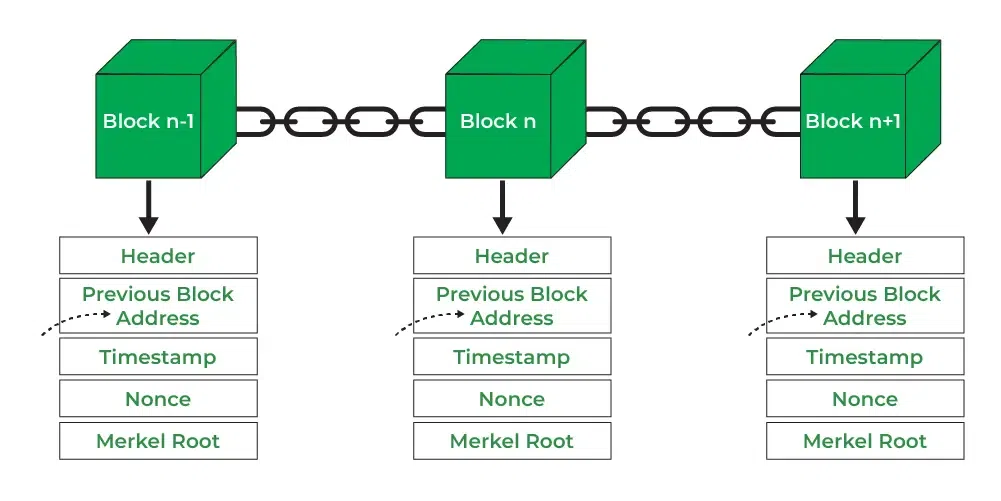
\includegraphics[width=0.8\textwidth]{blockchainstruct1.png}
\caption{ساختار عمومی زنجیره بلوکی: زنجیره‌ای از بلوک‌ها با اتصال هش هر بلوک به بلوک قبلی}
\label{fig:blockchain_struct}
\end{figure}

شکل \ref{fig:blockchain_struct} ساختار عمومی زنجیره بلوکی و نحوه اتصال هر بلوک با هش بلوک قبلی را نشان می‌دهد.

\subsubsection{مکانیزم‌های توافق}

مکانیزم‌های توافق نقش حیاتی در عملکرد زنجیره بلوکی ایفا می‌کنند \cite{razaBlockchainBasedReputationTrust2024}:

\begin{table}[H]
\centering
\caption{مکانیزم‌های توافق در زنجیره بلوکی}
\label{tab:consensus}
\begin{tabular}{p{2.5cm} p{4cm} p{2.5cm} p{2.5cm}}
\toprule
\textbf{الگوریتم} & \textbf{ویژگی کلیدی} & \textbf{مصرف انرژی} & \textbf{مقیاس‌پذیری} \\
\midrule
\lr{PoW} & پازل محاسباتی & بسیار بالا & پایین \\
\lr{PoS} & مبتنی بر سهام اقتصادی & پایین & متوسط \\
\lr{DPoS} & رأی‌دهی به ازای هر سهم & پایین & بالا \\
\lr{PBFT} & پیچیدگی چندجمله‌ای & پایین & متوسط \\
\bottomrule
\end{tabular}
\end{table}

\subsection{چالش‌های زنجیره بلوکی در شبکه خودرویی}

فناوری زنجیره بلوکی با چالش‌های متعددی مواجه است \cite{razaBlockchainBasedReputationTrust2024}:

\begin{itemize}
  \item \textbf{مقیاس‌پذیری پایین:} تعداد محدود تراکنش‌ها در ثانیه (بیت‌کوین: ۷، اتریوم: ۱۵).
  \item \textbf{مصرف انرژی بالا:} الگوریتم اثبات کار نیازمند منابع محاسباتی قابل توجه است.
  \item \textbf{تأخیر بالا:} زمان تأیید تراکنش‌ها برای کاربردهای بلادرنگ مناسب نیست.
  \item \textbf{هزینه تراکنش:} وجود کارمزد برای هر تراکنش.
  \item \textbf{محدودیت ذخیره‌سازی:} حجم زیاد داده‌ها برای ذخیره‌سازی در زنجیره بلوکی.
  \item \textbf{حمله ۵۱ درصد:} مهاجم با اکثریت توان هش می‌تواند خرج دوباره و بازآرایی دفتر کل انجام دهد.
  \item \textbf{حریم خصوصی و همکاری‌پذیری:} مشکلات کیف پول و ادغام با سیستم‌های موجود.
\end{itemize}

\subsection{مزایا و کاربردهای زنجیره بلوکی در شبکه اقتضایی خودرویی}

زنجیره بلوکی با ویژگی‌های منحصربه‌فرد خود می‌تواند بسیاری از مشکلات شبکه اقتضایی خودرویی را حل کند \cite{razaBlockchainBasedReputationTrust2024, fengBPASBlockchainAssistedPrivacyPreserving2020, ghovanlooyghajarSBTMSScalableBlockchain2021}:

\begin{itemize}
  \item \textbf{غیرمتمرکزسازی:} حذف نقطه شکست منفرد و افزایش امنیت و تاب‌آوری.
  \item \textbf{تغییرناپذیری:} داده‌ها قابل تغییر یا دستکاری نیستند.
  \item \textbf{ردیابی:} جلوگیری از استفاده نادرست از داده‌ها از طریق تاریخچه کامل تراکنش‌ها.
  \item \textbf{شفافیت:} ثبت شفاف تراکنش‌ها.
  \item \textbf{قراردادهای هوشمند:} اجرای خودکار سیاست‌های امنیتی، از جمله ابطال مبتنی بر قرارداد هوشمند.
\end{itemize}

زنجیره بلوکی در حوزه‌های مختلف شبکه اقتضایی خودرویی کاربرد دارد \cite{razaBlockchainBasedReputationTrust2024, hozouriOverviewVANETVehicular2023}:

\begin{itemize}
  \item \textbf{افزایش امنیت:} تعیین صحت پیام‌های پخش‌شده بین خودروها.
  \item \textbf{حریم خصوصی:} رمزنگاری کلید عمومی برای محافظت از داده‌های حساس.
  \item \textbf{مدیریت اعتماد:} ذخیره مقادیر اعتماد در زنجیره بلوکی.
  \item \textbf{مدیریت هویت:} مدیریت غیرمتمرکز کلیدها و گواهی‌نامه‌ها.
  \item \textbf{ردیابی خودرو:} جلوگیری از دستکاری کیلومترشمار.
\end{itemize}

\subsection{راهکارهای رفع محدودیت‌های زنجیره بلوکی}

برای رفع محدودیت‌های زنجیره بلوکی در شبکه اقتضایی خودرویی، راهکارهای مختلفی ارائه شده است \cite{ghovanlooyghajarSBTMSScalableBlockchain2021, razaBlockchainBasedReputationTrust2024}:

\begin{itemize}
  \item \textbf{شاردینگ:} تقسیم شبکه به بخش‌های کوچکتر برای افزایش مقیاس‌پذیری.
  \item \textbf{الگوریتم‌های توافق جایگزین:} استفاده از \lr{PoS}، \lr{DPoS} و \lr{PBFT} به جای \lr{PoW}.
  \item \textbf{زنجیره‌های فرعی:} استفاده از زنجیره‌های فرعی برای کاهش بار شبکه اصلی.
  \item \textbf{لایه‌های مقیاس‌پذیری:} استفاده از لایه‌های مقیاس‌پذیری مانند \lr{Lightning Network}.
\end{itemize}

\subsubsection{سیستم مدیریت اعتماد مقیاس‌پذیر مبتنی بر زنجیره بلوکی \lr{(SBTMS)}}

سیستم \lr{SBTMS} یکی از راهکارهای نوین برای حل مشکلات زنجیره بلوکی در شبکه‌ی اقتضایی خودرویی است \cite{ghovanlooyghajarSBTMSScalableBlockchain2021}:

\begin{itemize}
  \item \textbf{معماری غیرمتمرکز:} استفاده از زنجیره بلوکی برای ایجاد پلتفرم غیرمتمرکز.
  \item \textbf{الگوریتم شاردینگ:} تقسیم شبکه به بخش‌های کوچکتر برای مقیاس‌پذیری.
  \item \textbf{استنباط بیزی:} محاسبه اعتماد بر اساس فرمول‌های بیزی.
  \item \textbf{پروتکل \lr{PBFT}:} پروتکل تحمل خطای بیزانس عملی.
\end{itemize}

نتایج شبیه‌سازی \lr{SBTMS} نشان می‌دهد که الگوریتم شاردینگ زمان تولید بلوک را به صورت تقریباً خطی افزایش می‌دهد، در حالی که در الگوریتم \lr{PoW} این زمان به صورت نمایی افزایش می‌یابد \cite{ghovanlooyghajarSBTMSScalableBlockchain2021}.

\subsection{\lr{IOTA Tangle} به عنوان جایگزین}

\lr{IOTA Tangle} یک فناوری دفتر کل توزیع‌شده \LTRfootnote{\lr{Distributed Ledger Technology (DLT)}} است که بر اساس ساختار گراف جهت‌دار بدون دور \LTRfootnote{\lr{Directed Acyclic Graph (DAG)}} طراحی شده است \cite{IOTATANGLE20, silvanoIotaTangleCryptocurrency2020}. برخلاف زنجیره بلوک‌های سنتی که از زنجیره بلوک‌ها استفاده می‌کنند، \lr{IOTA Tangle} از ساختار \lr{Tangle} استفاده می‌کند که در آن هر تراکنش جدید به دو تراکنش قبلی ارجاع می‌دهد \cite{silvanoIotaTangleCryptocurrency2020}. نسخه دوم این فناوری (\lr{IOTA Tangle V2.0}) با حذف هماهنگ‌کننده متمرکز و معرفی پروتکل‌های جدید اجماع، به مقیاس‌پذیری و غیرمتمرکزسازی واقعی دست یافته است \cite{sealeyIOTATangle202022}.

\begin{figure}[H]
\centering
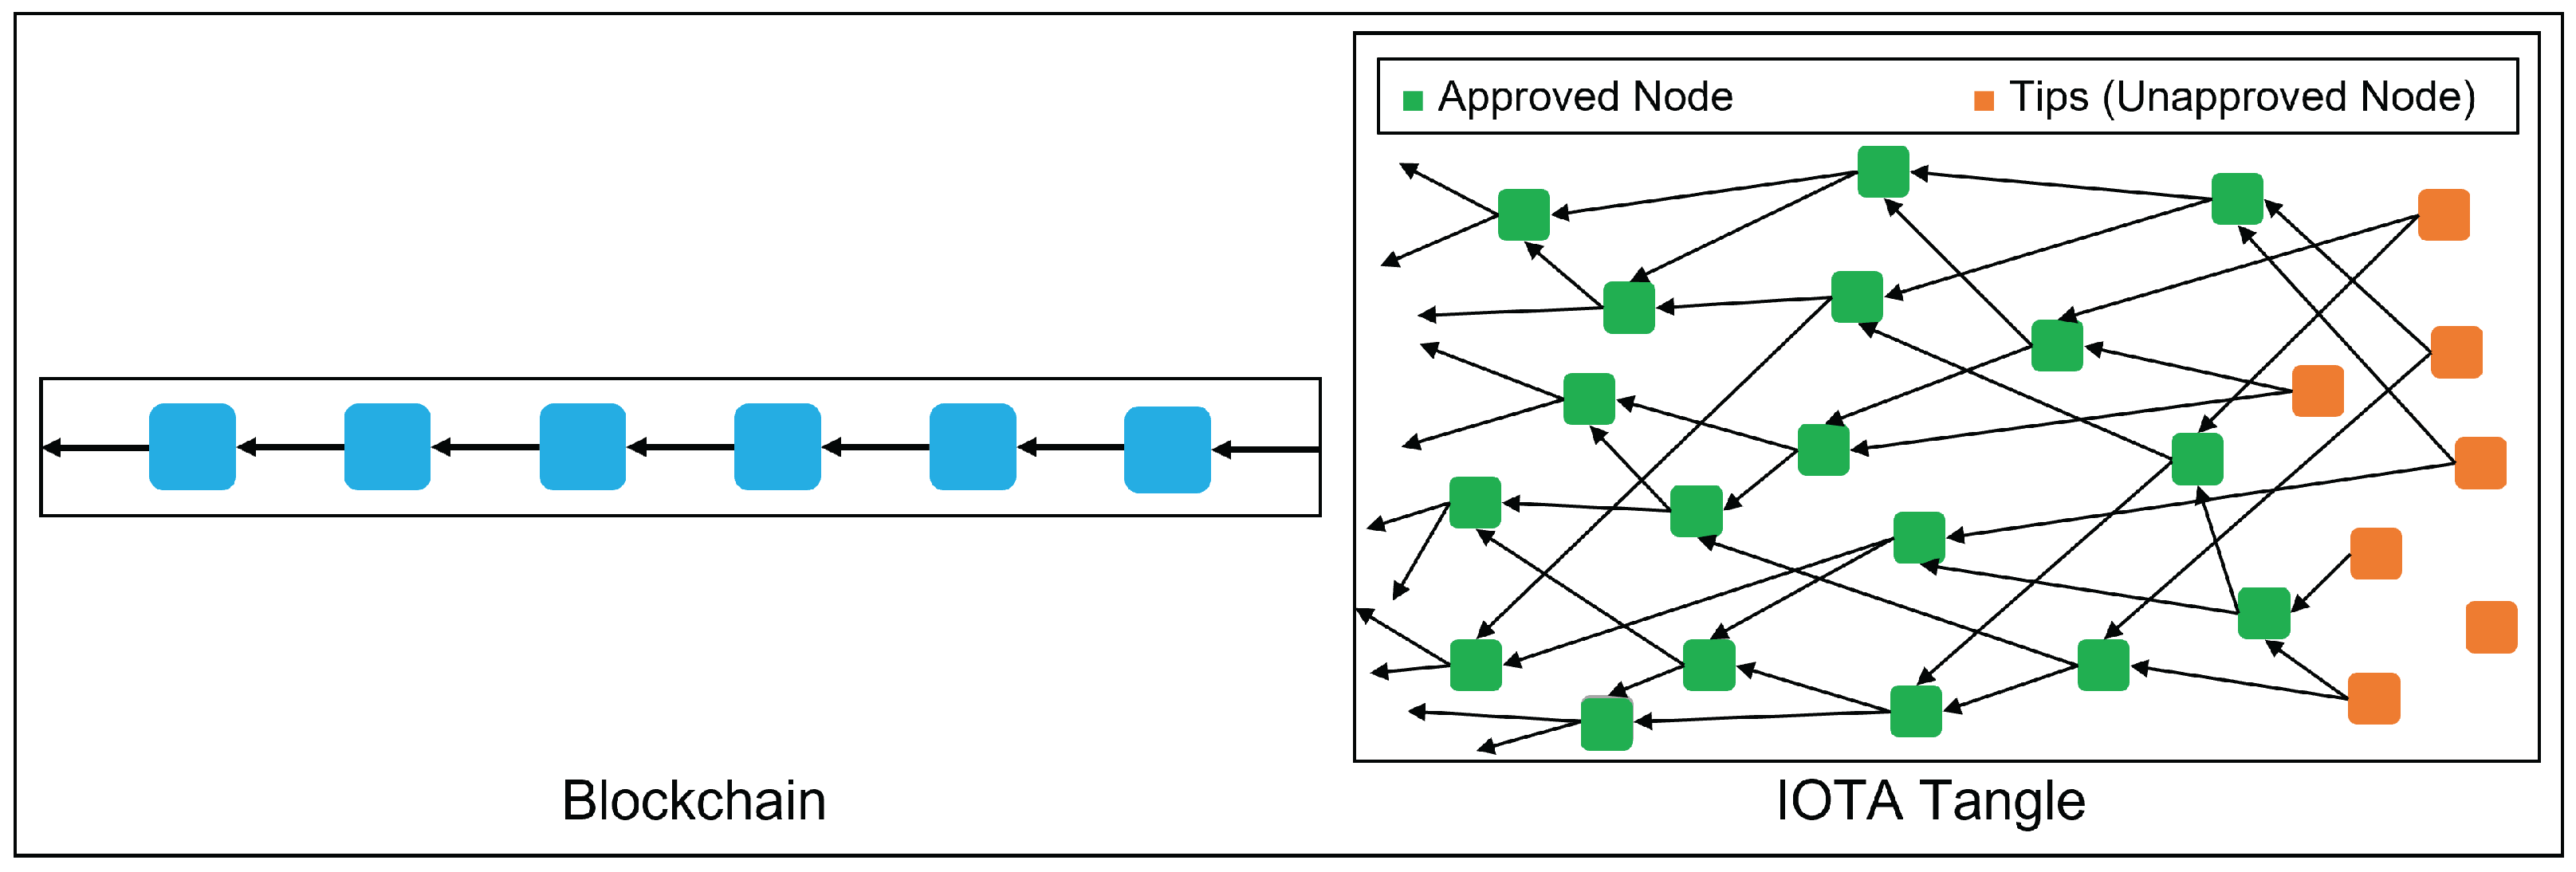
\includegraphics[width=0.95\textwidth]{IOTA vs Blockchain.png}
\caption{مقایسه تصویری \lr{IOTA Tangle} با زنجیره بلوکی سنتی}
\label{fig:iota_vs_bc}
\end{figure}

\lr{IOTA Tangle} به عنوان جایگزینی برای زنجیره بلوک، مشکلات اصلی آن در شبکه‌ی اقتضایی خودرویی را رفع می‌کند \cite{IOTATANGLE20, silvanoIotaTangleCryptocurrency2020}. در \lr{IOTA Tangle V2.0} سه لایه معماری وجود دارد \cite{IOTATANGLE20}:

\begin{enumerate}
  \item \textbf{لایه شبکه:} مدیریت عملیات سطح بایت و مبادلات همتا به همتا.
  \item \textbf{لایه ارتباطات:} مدیریت پیام‌ها، انتخاب نکات و کنترل نرخ.
  \item \textbf{لایه کاربردی:} اجرای بارهای پیام و اجرای توافق.
\end{enumerate}

از مهمترین ویژگی‌های \lr{IOTA Tangle V2.0} می‌توان به موارد زیر اشاره کرد \cite{IOTATANGLE20, sealeyIOTATangle202022}:

\begin{itemize}
  \item \textbf{مقیاس‌پذیری بالا:} با افزایش تراکنش‌ها، شبکه قوی‌تر شده و تأییدها سریع‌تر انجام می‌شوند.
  \item \textbf{بدون کارمزد:} تراکنش‌ها بدون هیچ هزینه‌ای انجام می‌شوند.
  \item \textbf{توافق غیرمتمرکز:} استفاده از پروتکل \lr{FPC}.
  \item \textbf{قراردادهای هوشمند:} پشتیبانی از قراردادهای هوشمند از طریق \lr{ISCP}.
  \item \textbf{امضای \lr{Ed25519}:} استفاده از طرح امضای کارآمد و ایمن. (توجه: این امضا کلاسیک است و در برابر محاسبات کوانتومی مقاوم نیست \cite{rahmawatiagustinaSystematicLiteratureReview2025}.)
\end{itemize}

برای مقایسه، تفاوت‌های اصلی \lr{IOTA Tangle} و زنجیره بلوکی در جدول \ref{tab:iota_vs_bc} نشان داده شده است:

\begin{table}[H]
\centering
\caption{مقایسه \lr{IOTA Tangle} با زنجیره بلوکی}
\label{tab:iota_vs_bc}
\begin{tabular}{p{3.5cm} p{4.5cm} p{4.5cm}}
\toprule
\textbf{ویژگی} & \textbf{زنجیره بلوکی} & \textbf{\lr{IOTA Tangle}} \\
\midrule
ساختار & زنجیره بلوک‌ها & گراف جهت‌دار بدون دور \\
کارمزد & بالا & بدون کارمزد \\
\lr{TPS} & پایین (۷-۱۵) & بالا و مقیاس‌پذیر \\
مصرف انرژی & بالا & پایین \\
ماینر & نیاز دارد & نیاز ندارد \\
\bottomrule
\end{tabular}
\end{table}

\lr{IOTA Tangle} در شبکه اقتضایی خودرویی کاربردهای زیر را دارد \cite{feraudoDIVADIDbasedReputation2024, silvanoIotaTangleCryptocurrency2020}:

\begin{itemize}
  \item \textbf{ذخیره‌سازی امتیازات شهرت:} ذخیره ایمن امتیازات شهرت خودروها.
  \item \textbf{تراکنش‌های بدون کارمزد:} امکان تبادل اطلاعات بدون هزینه.
  \item \textbf{تأیید سریع:} تأیید سریع تراکنش‌ها برای کاربردهای بلادرنگ.
  \item \textbf{امنیت سخت‌افزاری:} استفاده از امضای \lr{Ed25519} برای امنیت بالا.
\end{itemize}


% ========================================================================
% فصل ۹: مدیریت هویت و طرح‌های تصدیق هویت
% ========================================================================
\section{مدیریت هویت و طرح‌های تصدیق هویت}

\subsection{مدیریت هویت چیست و تکامل آن}

مدیریت هویت فرآیند شناسایی، تصدیق هویت و مدیریت دسترسی کاربران به سیستم‌ها و سرویس‌ها است \cite{mazzocca2025survey}. در شبکه اقتضایی خودرویی، مدیریت هویت نقش حیاتی در تضمین امنیت و حریم خصوصی ایفا می‌کند.

مدیریت هویت در طول زمان تکامل یافته است \cite{mazzocca2025survey}:

\begin{enumerate}
  \item \textbf{هویت متمرکز (۱۹۸۸-۱۹۹۸):} کنترل مرکزی توسط یک مرجع واحد.
  \item \textbf{هویت فدرالی (۱۹۹۸-۲۰۰۵):} ورود یکپارچه به سرویس‌های مختلف.
  \item \textbf{هویت کاربرمحور (۲۰۰۵-۲۰۱۲):} مدیریت مستقل هویت توسط کاربر.
  \item \textbf{هویت خودمختار (۲۰۱۲ تا کنون):} کنترل کامل کاربر بر داده‌های خود.
\end{enumerate}

\subsection{هویت خودمختار \lr{(SSI)}}

هویت خودمختار یک رویکرد نوین در مدیریت هویت است که به کاربران کنترل کامل بر داده‌های شخصی خود را می‌دهد \cite{mazzocca2025survey}. هویت خودمختار بر اساس فناوری‌های دفتر کل توزیع‌شده، شناسه‌های غیرمتمرکز و اعتبارنامه‌های تأییدپذیر ساخته شده است.

\begin{figure}[H]
\centering
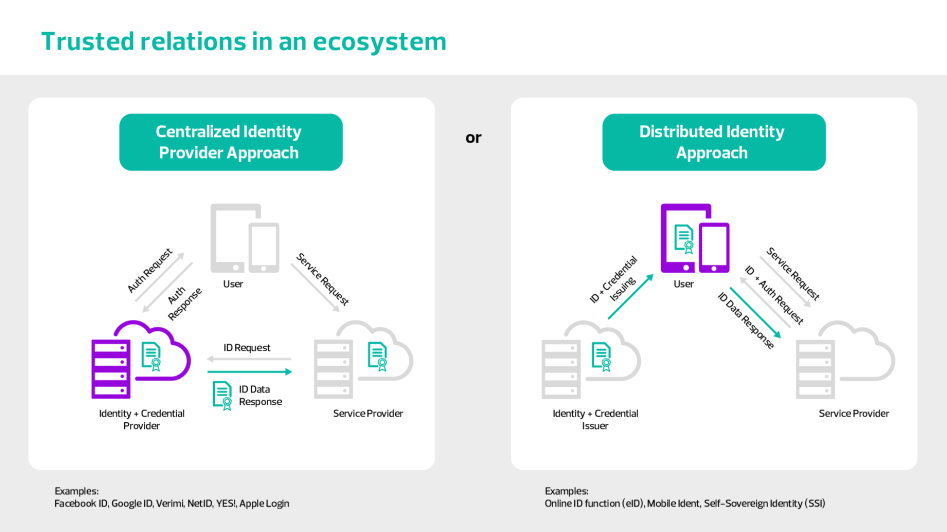
\includegraphics[width=0.85\textwidth]{SSI vs centeralized.png}
\caption{مقایسه معماری مدیریت هویت متمرکز و هویت خودمختار}
\label{fig:ssi_vs_centralized}
\end{figure}

دلایل مطرح شدن هویت خودمختار عبارتند از:

\begin{itemize}
  \item \textbf{نقطه شکست منفرد:} سیستم‌های متمرکز در برابر حملات آسیب‌پذیر هستند.
  \item \textbf{نقض حریم خصوصی:} نقض داده‌ها در سیستم‌های متمرکز رایج است.
  \item \textbf{کنترل محدود کاربر:} کاربران کنترل محدودی بر داده‌های خود دارند.
  \item \textbf{نیاز به حریم خصوصی:} افزایش نگرانی‌ها در مورد حریم خصوصی داده‌ها.
\end{itemize}

\subsection{شناسه‌های غیرمتمرکز \lr{(DID)}}

شناسه‌های غیرمتمرکز شناسه‌های جهانی منحصربه‌فردی هستند که بدون نیاز به مرجع مرکزی عمل می‌کنند \cite{mazzocca2025survey}. مثال:
\begin{center}
\texttt{\lr{did:example:123456789abcdefghi}}
\end{center}

معماری شناسه‌های غیرمتمرکز شامل اجزای زیر است \cite{mazzocca2025survey}:

\begin{itemize}
  \item \textbf{شناسه غیرمتمرکز:} شناسه جهانی منحصربه‌فرد.
  \item \textbf{سند شناسه غیرمتمرکز:} سند \lr{JSON-LD} حاوی کلیدهای عمومی و نقاط اتصال سرویس.
  \item \textbf{روش شناسه غیرمتمرکز:} مشخص‌کننده نحوه ایجاد، حل، به‌روزرسانی و غیرفعال کردن شناسه غیرمتمرکز.
  \item \textbf{ثبات داده تأییدپذیر:} مخزن ذخیره‌سازی اسناد شناسه غیرمتمرکز.
\end{itemize}

انواع شناسه‌های غیرمتمرکز:

\begin{itemize}
  \item \textbf{بی‌طرفه \LTRfootnote{Anywise}:} قابل استفاده با طرف‌های نامشخص.
  \item \textbf{دوتایی \LTRfootnote{Pairwise}:} فقط توسط شخص و یک طرف دیگر شناخته شده.
  \item \textbf{چندطرفه \LTRfootnote{N-wise}:} توسط دقیقاً \lr{N} طرف شناخته شده.
\end{itemize}

\subsection{اعتبارنامه‌های تأییدپذیر \lr{(VC)}}

اعتبارنامه‌های تأییدپذیر مدارک الکترونیکی رمزنگاری‌شده و تغییرناپذیر هستند که توسط \lr{W3C} استانداردسازی شده‌اند \cite{mazzocca2025survey}.

بازیگران اصلی اعتبارنامه‌های تأییدپذیر عبارتند از:

\begin{itemize}
  \item \textbf{نگهدارنده\LTRfootnote{Holder}:} موجودیتی که اعتبارنامه تأییدپذیر را کنترل می‌کند.
  \item \textbf{صادرکننده\LTRfootnote{Issuer}:} نهاد معتبری که اعتبارنامه تأییدپذیر را صادر می‌کند.
  \item \textbf{تأییدکننده\LTRfootnote{Verifier}:} موجودیتی که به اعتبارنامه تأییدپذیر نیاز دارد.
\end{itemize}

افشای انتخابی اطلاعات اعتبارنامه‌ها با استفاده از اثبات دانش صفر\LTRfootnote{\lr{Zero-knowledge proofs}} انجام می‌شود.

\subsection{مشکلات امنیتی رفع‌شده توسط \lr{SSI} و \lr{DID}}

فناوری‌های شناسه‌های غیرمتمرکز و هویت خودمختار مشکلات زیر را در شبکه اقتضایی خودرویی رفع می‌کنند \cite{mazzocca2025survey, feraudoDIVADIDbasedReputation2024}:

\begin{itemize}
  \item \textbf{حذف نقطه شکست منفرد:} حذف مرجع متمرکز با استفاده از شناسه‌های غیرمتمرکز.
  \item \textbf{حفظ حریم خصوصی:} استفاده از شناسه‌های غیرمتمرکز به عنوان شبه‌نام و افشای انتخابی.
  \item \textbf{قابلیت ردیابی شرطی:} امکان شناسایی هویت واقعی در صورت نیاز.
  \item \textbf{مدیریت شهرت غیرمتمرکز:} ذخیره امتیازات شهرت به صورت غیرمتمرکز.
  \item \textbf{مقابله با حملات تقلید و حملات سیبل:} یک شناسه غیرمتمرکز برای هر خودرو.
\end{itemize}

\subsection{طرح‌های موجود برای تصدیق هویت}

شبه‌نام یکی از مهمترین چالش‌ها در حفظ حریم خصوصی شبکه اقتضایی خودرویی است \cite{luPseudonymChangingSocial2012, al-aniPrivacySafetyImprovement2023, rahmawatiagustinaSystematicLiteratureReview2025}. راهکارهای موجود عبارتند از:

\subsubsection{تغییر شبه‌نام در نقاط اجتماعی \lr{(PCS)}}

رویکرد \lr{PCS} پیشنهاد می‌کند که خودروها شبه‌نام خود را در نقاط اجتماعی تغییر دهند \cite{luPseudonymChangingSocial2012}:

\begin{itemize}
  \item نقاط اجتماعی مکان‌هایی هستند که چندین خودرو در آن‌ها جمع می‌شوند.
  \item مانند تقاطع‌های چراغ قرمز یا پارکینگ‌های رایگان.
  \item با تغییر هم‌زمان شبه‌نام در این نقاط، حریم خصوصی افزایش می‌یابد.
\end{itemize}

\subsubsection{طرح حریم خصوصی مرتبط با ایمنی \lr{(SRPS)}}

طرح \lr{SRPS} تعادلی بین حریم خصوصی و ایمنی ایجاد می‌کند \cite{al-aniPrivacySafetyImprovement2023}:

\begin{itemize}
  \item \textbf{کاهش دوره‌های سکوت:} خودرو در صورت پیش‌بینی تصادف از سکوت خارج می‌شود.
  \item \textbf{تغییر هوشمند شبه‌نام:} استفاده از الگوریتم ردیابی چندهدفه.
  \item \textbf{حفظ ایمنی:} نزدیک به ۱۰ پیام ایمنی در ثانیه.
  \item \textbf{کاهش ردیابی:} تا ۲۰ درصد در تراکم بالا.
\end{itemize}

\subsubsection{سیستم شناسه‌های غیرمتمرکز مبتنی بر شهرت \lr{(DIVA)}}

سیستم \lr{DIVA} ترکیبی از شناسه‌های غیرمتمرکز و \lr{IOTA Tangle} برای مدیریت شهرت در شبکه اقتضایی خودرویی است \cite{feraudoDIVADIDbasedReputation2024}:

\begin{itemize}
  \item استفاده از شناسه‌های غیرمتمرکز برای شناسایی خودروها.
  \item ذخیره امتیازات شهرت در \lr{IOTA Tangle}.
  \item محاسبه امتیازات شهرت بر اساس پیام‌های ایمنی و غیرایمنی.
  \item شناسایی دقیق مشارکت‌کنندگان موذی با دقت تقریباً ۹۰ درصد.
\end{itemize}

\begin{figure}[H]
\centering
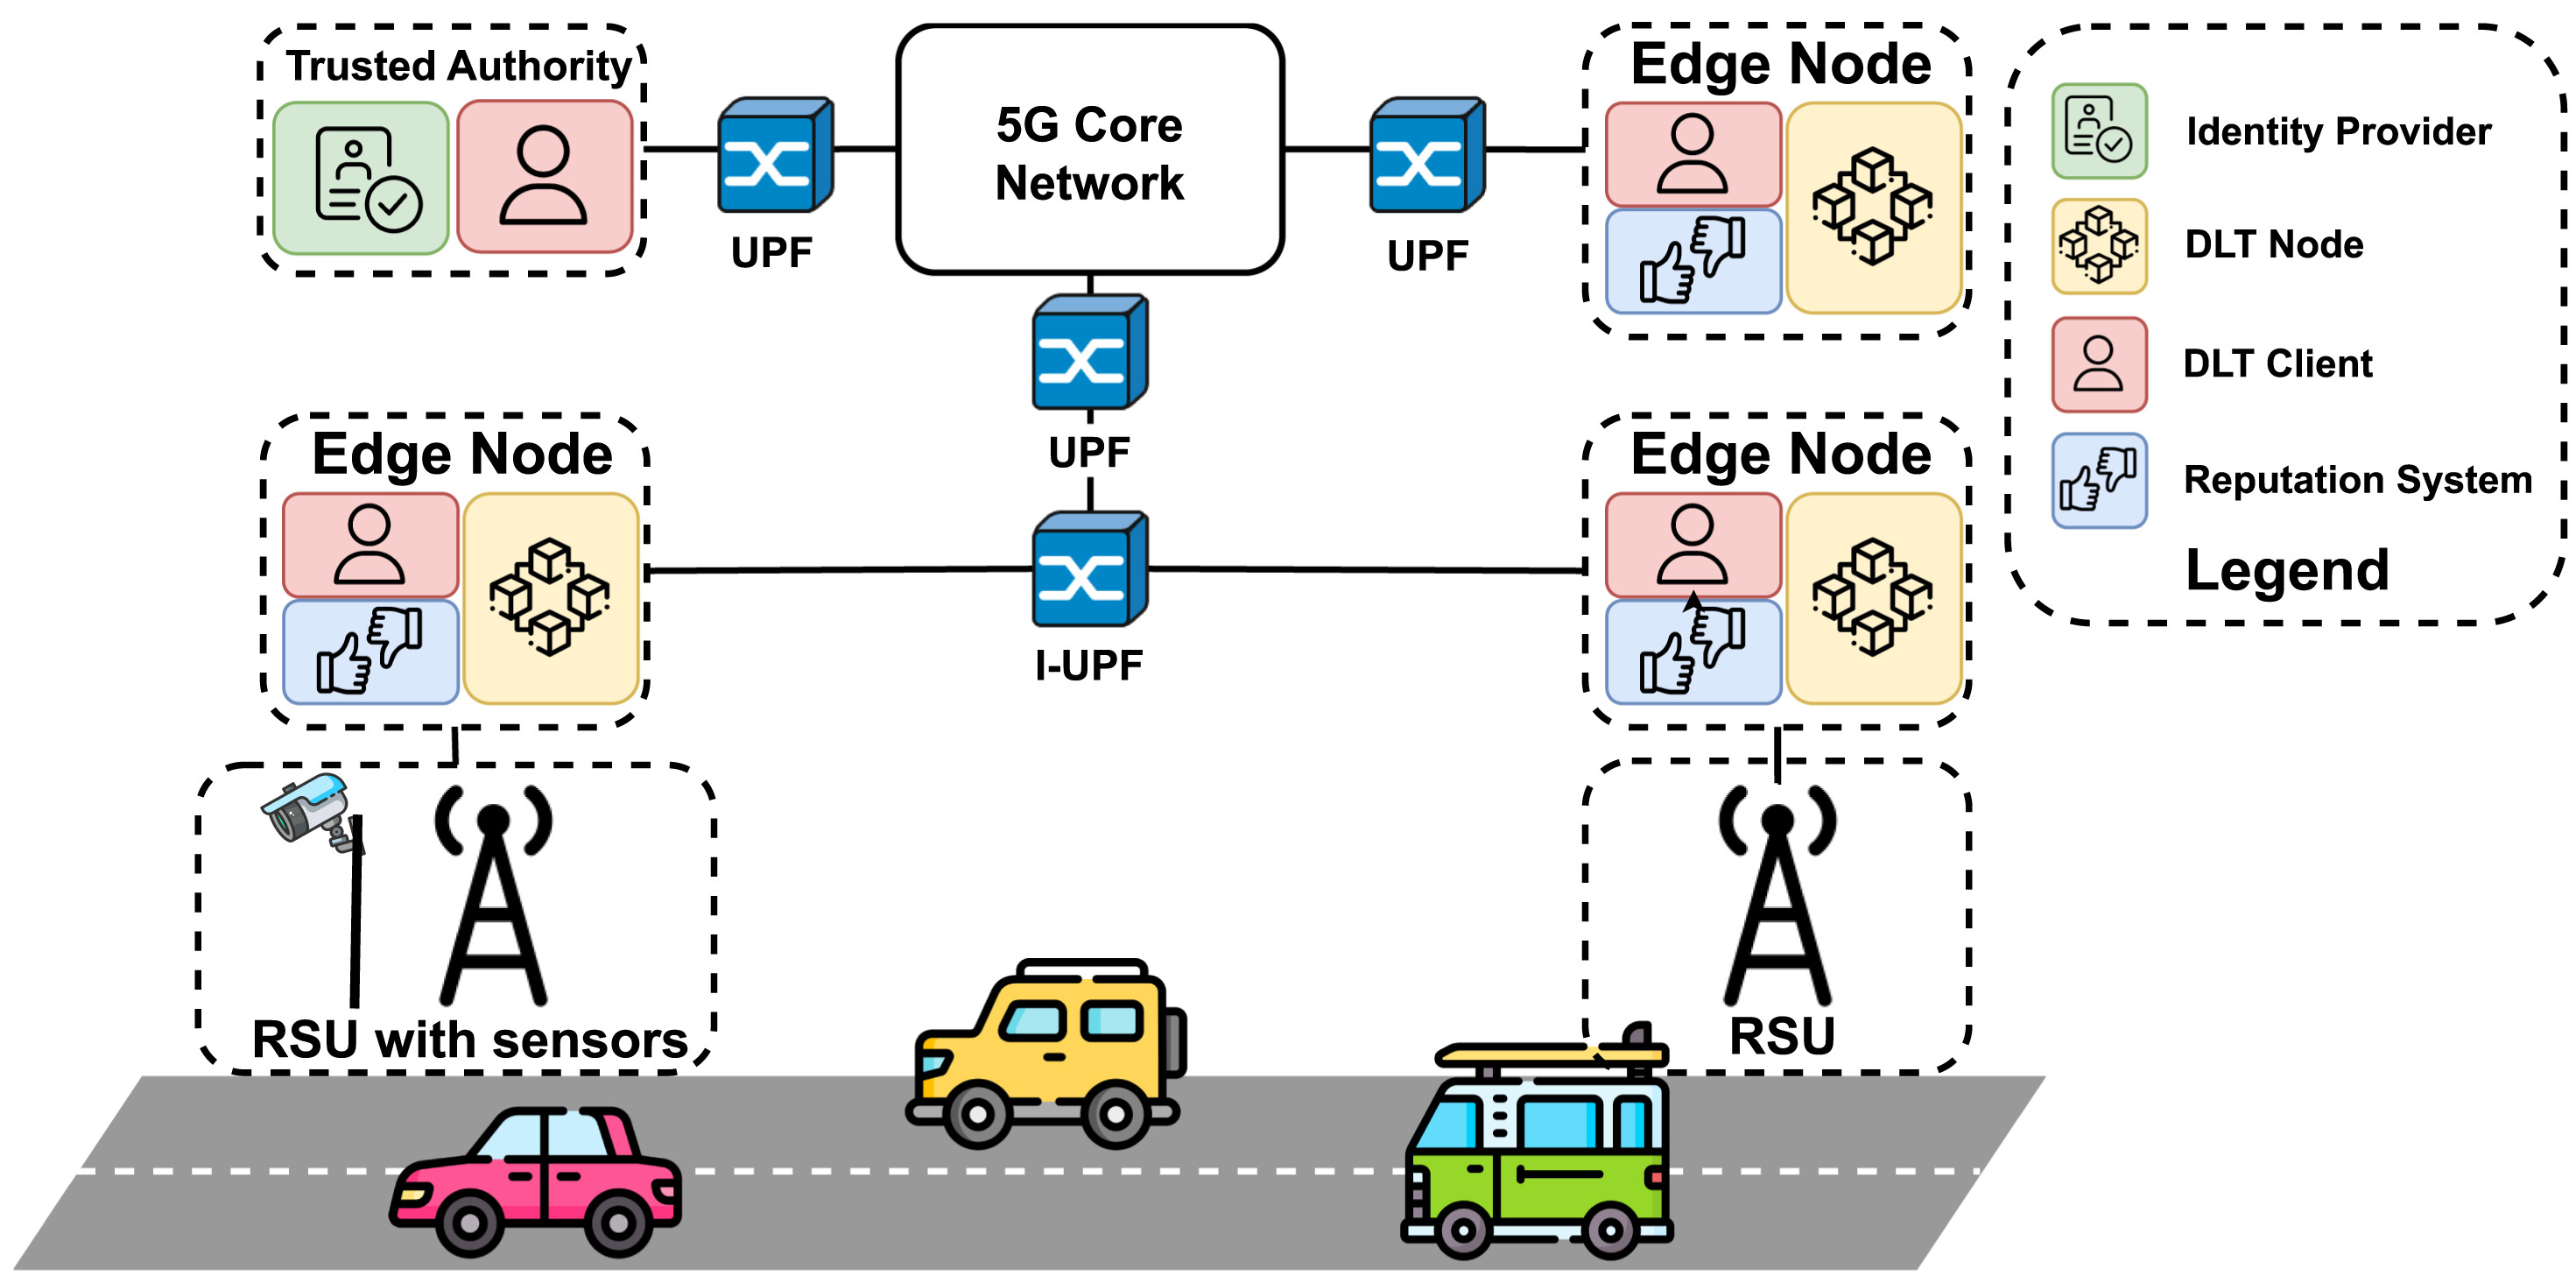
\includegraphics[width=0.9\textwidth]{DIVA.jpg}
\caption{معماری سیستم \lr{DIVA}: سیستم شهرت مبتنی بر شناسه‌های غیرمتمرکز برای انتقال امن در شبکه اقتضایی خودرویی با استفاده از \lr{IOTA Tangle}}
\label{fig:diva_arch}
\end{figure}

\subsubsection{پروتکل‌های امنیتی مبتنی بر زنجیره بلوکی}

چندین پروتکل امنیتی مبتنی بر زنجیره بلوکی برای شبکه اقتضایی خودرویی پیشنهاد شده است:

\paragraph{سیستم تصدیق هویت مبتنی بر زنجیره بلوکی \lr{(BPAS)}:}
سیستم \lr{BPAS} چارچوبی نوین برای تصدیق هویت غیرمتمرکز در شبکه اقتضایی خودرویی ارائه می‌دهد \cite{fengBPASBlockchainAssistedPrivacyPreserving2020}:

\begin{itemize}
  \item \textbf{بدون نیاز به مرکز ثبت آنلاین:} فقط در مرحله راه‌اندازی.
  \item \textbf{پیگیری شرطی:} امکان شناسایی خودروهای موذی.
  \item \textbf{لغو پویا:} لغو دسترسی خودروهای متخلف.
  \item \textbf{پیاده‌سازی بر \lr{Hyperledger Fabric}:} عملکرد بالا و مقیاس‌پذیر.
\end{itemize}

\paragraph{تصدیق هویت ناشناس مبتنی بر زنجیره بلوکی \lr{(BAIV)}:}
طرح \lr{BAIV} تصدیق هویت ناشناس و حفظ یکپارچگی پیام را ترکیب می‌کند \cite{mariaBAIVEfficientBlockchainBased2022}:

\begin{itemize}
  \item \textbf{انتقال ایمن:} تصدیق هویت بدون مرجع قابل اعتماد.
  \item \textbf{حریم خصوصی شرطی:} لغو خودروهای موذی در صورت اختلاف.
  \item \textbf{حفظ یکپارچگی:} جلوگیری از دستکاری پیام‌ها.
  \item \textbf{کارایی بالا:} استفاده از رمزنگاری منحنی بیضوی.
\end{itemize}

\paragraph{پروتکل امنیتی و حفظ حریم خصوصی \lr{(GSIS)}:}
پروتکل \lr{GSIS} ترکیبی از امضای گروهی و امضای مبتنی بر هویت ارائه می‌دهد \cite{linGSISSecurePrivacyPreserving2007}:

\begin{itemize}
  \item \textbf{حریم خصوصی شرطی:} حفظ حریم خصوصی با امکان پیگیری در صورت نیاز.
  \item \textbf{تصدیق هویت ناشناس:} ارسال پیام‌ها به صورت ناشناس.
  \item \textbf{ساده‌سازی مدیریت گواهی‌نامه:} استفاده از هر رشته به عنوان کلید عمومی معتبر.
\end{itemize}

% ========================================================================
% فصل ۱۰: هوش مصنوعی و تشخیص ناهنجاری
% ========================================================================
\section{هوش مصنوعی و تشخیص ناهنجاری}
روش‌های هوش مصنوعی و یادگیری ماشین نقش مهمی در تقویت امنیت شبکه اقتضایی خودرویی ایفا می‌کنند \cite{farsimadanReviewSecurityChallenges2025}. این روش‌ها در چهار حوزه اصلی زیر دسته‌بندی می‌شوند:

\subsection{تشخیص ناهنجاری و حملات}
شبکه‌های عصبی \lr{CNN} و \lr{LSTM} برای شناسایی رفتارهای غیرعادی به کار می‌روند. همچنین، یادگیری بدون نظارت برای تشخیص حملات پارازیتی در لایه بی‌سیم و حملات بر \lr{CAN bus} در شبکه داخلی خودرو استفاده می‌شود.

\subsection{تحلیل آسیب‌پذیری و اعتماد}
تحلیل زنده ترافیک شبکه، آسیب‌پذیری‌ها را شناسایی می‌کند. منطق فازی نیز برای محاسبه اعتماد و تضمین دقت و یکپارچگی پیام‌های رویداد به کار گرفته می‌شود.

\subsection{یادگیری توزیع‌شده و تقویتی}
ترکیب زنجیره بلوکی و یادگیری فدرال، انتقال امن اطلاعات را با حفظ حریم خصوصی ممکن می‌سازد. یادگیری تقویتی نیز برای ارزیابی قابلیت اطمینان خودروهای رانندگی خودکار استفاده می‌شود.

\subsection{چالش‌ها}
یادگیری فدرال در برابر مسموم‌سازی داده و حملات تخاصمی آسیب‌پذیر است و به مکانیزم‌های مقاوم‌سازی نیاز دارد \cite{farsimadanReviewSecurityChallenges2025}.

% ========================================================================
% فصل ۱۱: فناوری‌های نوظهور
% ========================================================================
\section{فناوری‌های نوظهور}
فناوری‌های نوظهور در شبکه‌ی اقتضایی خودرویی (\lr{VANET}) با هدف کاهش تأخیر، افزایش مقیاس‌پذیری، بهبود مدیریت شبکه و تقویت امنیت به کار گرفته می‌شوند. این فناوری‌ها در شش حوزه اصلی دسته‌بندی می‌شوند:

\subsection{رایانش ابری، لبه و مه}
مدل‌های رایانش ابری و لبه\LTRfootnote{\lr{Cloud/Edge Computing}} با توزیع پردازش و ذخیره‌سازی، مقیاس‌پذیری شبکه را افزایش داده و بار محاسباتی گره‌های خودرویی را کاهش می‌دهند \cite{xuInternetVehiclesBig2018}. رایانش لبه با انتقال پردازش به نزدیکی منبع داده، تأخیر پاسخ‌گویی را به حداقل می‌رساند. معماری‌های مه\LTRfootnote{\lr{Fog Computing}} نیز به عنوان لایه میانی بین ابر و لبه، پردازش بلادرنگ را در لبه شبکه ممکن ساخته و برای کاربردهای حساس به تأخیر مانند هشدار تصادف و ترمز اضطراری مناسب هستند \cite{niSecuringFogComputing2018}. با این حال، توزیع‌شدگی این معماری‌ها معرض حمله را گسترش می‌دهد و نیازمند مکانیزم‌های امنیتی توزیع‌شده است.

\subsection{شبکه‌های نسل پنجم و ششم}
معماری امنیتی \lr{5G/6G} شامل مؤلفه‌های کلیدی \lr{AUSF} (کارگزار امنیت و تصدیق هویت)، \lr{SEAF} (کارگزار امنیت لبه) و \lr{ARPF} (تابع مخزن اعتبارنامه تصدیق هویت) است که به صورت بومی در معماری مبتنی بر سرویس\LTRfootnote{\lr{SBA}} طراحی شده‌اند \cite{farsimadanReviewSecurityChallenges2025}. شبکه‌سازی مبتنی بر سرویس امکان جداسازی عملکردهای شبکه و استقرار مستقل آن‌ها را فراهم می‌کند. با ظهور \lr{6G}، یکپارچگی هوش مصنوعی بومی، سطوح هوشمند قابل بازپیکربندی\LTRfootnote{\lr{RIS}} و ارتباطات تراهرتزی چالش‌های امنیتی جدیدی مانند حملات لایه فیزیکی پیشرفته و مدیریت هویت در مقیاس انبوه را مطرح می‌سازند.

\subsection{برش شبکه و مجازی‌سازی}
برش شبکه\LTRfootnote{\lr{Network Slicing}} امکان جداسازی منطقی منابع شبکه برای سرویس‌های مختلف (مانند ترافیک ایمنی، سرگرمی و مدیریت ناوگان) را فراهم می‌کند و ایزولاسیون امنیتی بین برش‌ها از نشت اطلاعات و حملات متقابل جلوگیری می‌نماید \cite{farsimadanReviewSecurityChallenges2025}. مجازی‌سازی توابع شبکه\LTRfootnote{\lr{NFV}} و شبکه‌های نرم‌افزارمحور\LTRfootnote{\lr{SDN}} نیز انعطاف‌پذیری در مدیریت، استقرار سریع سیاست‌های امنیتی و پاسخ پویا به تهدیدات را ممکن می‌سازند. با این حال، رابط‌های باز و کنترل‌کننده متمرکز، معرض حمله جدیدی ایجاد می‌کنند که نیازمند حفاظت ویژه است.

\subsection{شبکه‌های خودرویی نرم‌افزارمحور}
در شبکه‌های خودرویی نرم‌افزارمحور\LTRfootnote{\lr{SDVN}}، جداسازی صفحه کنترل از صفحه داده امکان مدیریت متمرکز و انعطاف‌پذیر ترافیک را فراهم می‌کند، اما امنیت کنترل‌کننده مرکزی به عنوان چالش اصلی مطرح است \cite{rahmawatiagustinaSystematicLiteratureReview2025}. حمله به کنترل‌کننده می‌تواند کل شبکه را مختل کند؛ بنابراین، افزونگی کنترل‌کننده، پروتکل‌های اجماع توزیع‌شده و رمزنگاری کانال کنترل ضروری است.

\subsection{معماری‌های ترکیبی}
ترکیب زنجیره بلوک، رایانش ابری و لبه برای تأمین هم‌زمان امنیت، شفافیت و مقیاس‌پذیری در \lr{VANET} استفاده می‌شود \cite{farsimadanReviewSecurityChallenges2025}. زنجیره بلوک ثبت غیرقابل انکار تراکنش‌ها و رویدادها را فراهم می‌کند، در حالی که لایه‌های ابر و لبه توان پردازشی لازم برای اجرای الگوریتم‌های اجماع و تحلیل بلادرنگ را تأمین می‌نمایند. این معماری‌ها برای کاربردهایی مانند مدیریت اعتماد توزیع‌شده، ثبت رویدادهای ایمنی و پرداخت‌های خودکار مناسب هستند.

\subsection{دوقلوهای دیجیتال و شبیه‌سازی بلادرنگ}
دوقلوهای دیجیتال\LTRfootnote{\lr{Digital Twins}} به عنوان بازنمایی مجازی از شبکه فیزیکی خودرویی، امکان شبیه‌سازی سناریوهای حمله، ارزیابی آسیب‌پذیری‌ها و آزمایش سیاست‌های امنیتی را بدون اختلال در شبکه واقعی فراهم می‌کنند. این فناوری برای پیش‌بینی رفتار شبکه تحت حملات و بهینه‌سازی استراتژی‌های دفاعی در حال ظهور است.

% ========================================================================
% فصل ۱۲: لایه سخت‌افزاری
% ========================================================================
\section{لایه سخت‌افزاری (بخش پشتیبان امنیت)}
لایه سخت‌افزاری به عنوان بخش پشتیبان امنیت، نقش مهمی در نگهداری کلیدها، تصدیق هویت دستگاه و مقابله با حملات فیزیکی ایفا می‌کند \cite{rahmawatiagustinaSystematicLiteratureReview2025}:

\subsection{ماژول پلتفرم قابل اعتماد}
ماژول پلتفرم قابل اعتماد\LTRfootnote{\lr{Trusted Platform Device, TPD}} یک سخت‌افزار امن است که نگهداری کلیدهای رمزنگاری، اجرای الگوریتم‌های رمزنگاری و تولید اعداد تصادفی امن را در محیطی ایزوله انجام می‌دهد. در \lr{VANET}، \lr{TPD} به عنوان لنگر اعتماد\LTRfootnote{\lr{Trust Anchor}} عمل می‌کند و از استخراج کلیدها حتی در صورت دسترسی فیزیکی مهاجم به خودرو جلوگیری می‌نماید. با این حال، هزینه استقرار \lr{TPD} در تمام خودروها و چالش‌های مدیریتی آن قابل توجه است.

\subsection{توابع فیزیکی غیرقابل شبیه‌سازی}
توابع فیزیکی غیرقابل شبیه‌سازی\LTRfootnote{\lr{Physically Unclonable Functions, PUF}} از نویز ذاتی و تغییرات فرآیند ساخت تراشه برای تولید اثر انگشت سخت‌افزاری منحصربه‌فرد استفاده می‌کنند. این اثر انگشت برای تصدیق هویت دستگاه بدون نیاز به ذخیره‌سازی کلید در حافظه غیرفرار به کار می‌رود. مزیت اصلی \lr{PUF} مقاومت در برابر حملات شبیه‌سازی و کپی‌برداری است، زیرا خواص فیزیکی تراشه قابل بازتولید نیستند.

\subsection{تصدیق چندعاملی}
تصدیق چندعاملی\LTRfootnote{\lr{Multi-Factor Authentication, MFA}} با ترکیب چندین عامل مستقل — رمز عبور (چیزی که کاربر می‌داند)، زیست‌سنجی (چیزی که کاربر هست) و سخت‌افزار امن (چیزی که کاربر دارد) — سطح امنیت دسترسی را به طور چشمگیری افزایش می‌دهد. در \lr{VANET}، ترکیب \lr{TPD} به عنوان عامل سخت‌افزاری با اعتبارنامه‌های دیجیتال و در صورت نیاز زیست‌سنجی راننده، از دسترسی غیرمجاز به سامانه‌های حیاتی خودرو جلوگیری می‌کند.

\subsection{مقابله با حملات کانال جانبی}
حملات کانال جانبی\LTRfootnote{\lr{Side-Channel Attacks}} با تحلیل نشتی‌های فیزیکی مانند توان مصرفی، تابش الکترومغناطیسی، زمان‌بندی اجرا و صوت، اطلاعات حساس مانند کلیدهای رمزنگاری را استخراج می‌کنند \cite{farsimadanReviewSecurityChallenges2025}. مقابله با این حملات شامل تکنیک‌هایی مانند متعادل‌سازی توان مصرفی، تصادفی‌سازی زمان‌بندی، پنهان‌سازی الکترومغناطیسی و طراحی مدارهای مقاوم در برابر دستکاری است. در خودروهای متصل، محافظت از \lr{TPD} و \lr{PUF} در برابر این حملات حیاتی است.

\subsection{عنصر امن سخت‌افزاری و محیط اجرای مطمئن}
علاوه بر \lr{TPD}، عناصر امن سخت‌افزاری\LTRfootnote{\lr{eSE}} و محیط‌های اجرای مطمئن\LTRfootnote{\lr{TEE}} مانند \lr{ARM TrustZone} و \lr{Intel SGX} برای ایزوله‌سازی عملیات حساس از سیستمعامل اصلی به کار می‌روند. \lr{TEE} امکان اجرای امن الگوریتم‌های رمزنگاری و پردازش داده‌های حساس را در محیطی ایزوله فراهم می‌کند، حتی اگر سیستمعامل اصلی آلوده شده باشد.

\subsection{ملاحظات هزینه و مدیریت}
استقرار سخت‌افزار امن در مقیاس ناوگان خودرویی هزینه قابل توجهی به همراه دارد و مدیریت چرخه عمر کلیدها، به‌روزرسانی میان‌افزار امن و تأمین زنجیره تولید از چالش‌های عملیاتی هستند \cite{rahmawatiagustinaSystematicLiteratureReview2025}. تعادل بین امنیت، هزینه و قابلیت استفاده باید در طراحی سامانه‌های خودرویی لحاظ شود.


% ========================================================================
% فصل ۱۳: مسائل باز و کارهای آینده
% ========================================================================
\section{مسائل باز و کارهای آینده}
بر اساس بررسی‌های انجام‌شده، مهم‌ترین مسائل باز در امنیت شبکه اقتضایی خودرویی و جهت‌گیری‌های پژوهشی برای رفع آن‌ها در حوزه‌های زیر دسته‌بندی می‌شوند \cite{farsimadanReviewSecurityChallenges2025, rahmawatiagustinaSystematicLiteratureReview2025}:

\subsection{معاوضه حریم خصوصی، امنیت و کارایی}
چالش مرکزی در طراحی سیستم‌های امنیتی \lr{VANET}، برقراری تعادل میان سه هدف متعارض است: حفظ حریم خصوصی کاربران، تأمین امنیت ارتباطات و تضمین کارایی سیستم. افزایش گمنامی معمولاً به قیمت کاهش قابلیت ردیابی و پاسخگویی تمام می‌شود، در حالی که مکانیزم‌های امنیتی قوی‌تر سربار محاسباتی و تأخیر بیشتری تحمیل می‌کنند.

\subsection{استراتژی تغییر شبه‌نام و چرخه حیات کامل آن}
هیچ استراتژی تغییر شبه‌نام واحدی وجود ندارد که در همه شرایط (تراکم ترافیک، سرعت خودرو، محیط شهری یا بزرگراهی) بهترین عملکرد را ارائه دهد \cite{rahmawatiagustinaSystematicLiteratureReview2025}. طراحی استراتژی‌های تطبیقی که بتوانند به صورت پویا با شرایط محیطی سازگار شوند، همچنان یک مسئله باز است. از این رو، پیاده‌سازی کامل چرخه حیات شبه‌نام — از تولید و توزیع تا تغییر، ابطال و ردیابی — بدون افت عملکرد سیستم، یک هدف کلیدی پژوهش‌های آینده است \cite{rahmawatiagustinaSystematicLiteratureReview2025}. این امر شامل یکپارچه‌سازی استراتژی‌های تغییر شبه‌نام با سایر مکانیزم‌های امنیتی است.

\subsection{اتکا به واحدهای کنارجاده‌ای و نقطه شکست منفرد}
وابستگی به واحدهای کنارجاده‌ای\LTRfootnote{\lr{RSU}} به عنوان گره‌های مورد اعتماد، نقطه شکست منفرد\LTRfootnote{\lr{Single Point of Failure, SPoF}} ایجاد می‌کند. حمله یا خرابی یک \lr{RSU} می‌تواند امنیت و دسترس‌پذیری بخش قابل توجهی از شبکه را مختل کند. کاهش این وابستگی و طراحی معماری‌های مقاوم در برابر خرابی \lr{RSU} ضروری است.

\subsection{مقیاس‌پذیری، محدودیت منابع و معماری‌های ترکیبی}
در ترافیک شهری متراکم با صدها خودرو در محدوده یک \lr{RSU}، مقیاس‌پذیری پروتکل‌های امنیتی به چالش کشیده می‌شود. محدودیت منابع محاسباتی واحدهای سوارشونده\LTRfootnote{\lr{OBU}} و واحدهای کنارجاده‌ای، اجرای الگوریتم‌های رمزنگاری سنگین و پروتکل‌های اجماع توزیع‌شده را با مشکل مواجه می‌کند. در این راستا، گسترش معماری‌های ترکیبی زنجیره بلوک، ابر و لبه برای تأمین هم‌زمان مقیاس‌پذیری و امنیت، یک مسیر پژوهشی فعال است؛ این معماری‌ها باید بتوانند تعادل مناسبی بین تمرکززدایی زنجیره بلوک و کارایی رایانش لبه برقرار کنند.

\subsection{واقع‌گرایی ارزیابی‌ها و مجموعه‌داده‌های باز}
بسیاری از ارزیابی‌های امنیتی در محیط‌های شبیه‌سازی‌شده با فرضیات ساده‌شده انجام می‌شوند. کمبود مجموعه‌داده‌های باز و واقعی از ترافیک \lr{VANET} و حملات واقعی، اعتبار نتایج را زیر سؤال می‌برد. بنابراین ایجاد و انتشار مجموعه‌داده‌های استاندارد و واقعی — شامل داده‌های بی‌سیم، ترافیک \lr{CAN bus} و رویدادهای امنیتی — و معیارهای ارزیابی یکپارچه برای اعتبارسنجی روش‌های امنیتی ضروری است.

\subsection{مقاومت مدل‌های یادگیری ماشین و یادگیری فدرال}
مدل‌های یادگیری ماشین به کار رفته در تشخیص ناهنجاری و تشخیص نفوذ، در برابر مسموم‌سازی داده\LTRfootnote{\lr{Data Poisoning}} و حملات تخاصمی\LTRfootnote{\lr{Adversarial Attacks}} آسیب‌پذیر هستند. مهاجم می‌تواند با تزریق نمونه‌های موذی به داده‌های آموزشی یا دستکاری ورودی‌ها در زمان استنتاج، مدل را فریب دهد. در این زمینه، توسعه روش‌های یادگیری فدرال مقاوم در برابر حملات تخاصمی و مسموم‌سازی داده، همراه با حفظ حریم خصوصی شرکت‌کنندگان، یک حوزه پژوهشی رو به رشد است؛ ترکیب یادگیری فدرال با حریم خصوصی تفاضلی\LTRfootnote{\lr{Differential Privacy}} و رمزنگاری همریخت\LTRfootnote{\lr{Homomorphic Encryption}} از مسیرهای امیدوارکننده است.

\subsection{آسیب‌پذیری‌های بی‌سیم و امنیت ارتباطات چندپرشی}
استراق سمع، حملات فردی در میان\LTRfootnote{\lr{Man-in-the-Middle}} و حملات \lr{Evil Twin} از جمله تهدیدات ذاتی کانال بی‌سیم هستند. در \lr{VANET} که ارتباطات با برد کوتاه و در محیط‌های متحرک انجام می‌شود، مقابله با این حملات دشوارتر است. از این رو، توسعه مکانیزم‌های بی‌سیم مقاوم برای امنیت ارتباطات چندپرشی\LTRfootnote{\lr{Multi-hop Communication}} در لایه‌های مختلف \lr{ITS}، از نیازهای پژوهشی است \cite{VanetSecurityPrivacy}.

\subsection{امضاهای دیجیتال سریع و سبک}
طرح‌های امضای دیجیتال موجود یا سرعت کافی برای کاربردهای بلادرنگ ایمنی را ندارند یا از نظر محاسباتی برای واحدهای سوارشونده با منابع محدود سنگین هستند. طراحی و استانداردسازی امضاهای سبک و سریع که امنیت کافی را نیز حفظ کنند، همچنان یک نیاز برآورده‌نشده است؛ طرح‌های مبتنی بر منحنی‌های بیضوی سبک، امضاهای تجمعی و امضاهای کوتاه از جمله گزینه‌های مورد بررسی هستند.

\subsection{تهدید محاسبات کوانتومی و رمزنگاری پساکوانتومی}
پیشرفت رایانه‌های کوانتومی، الگوریتم‌های رمزنگاری مبتنی بر \lr{RSA} و \lr{ECC} را در معرض خطر قرار می‌دهد \cite{rahmawatiagustinaSystematicLiteratureReview2025}. آمادگی برای گذار به رمزنگاری پساکوانتومی\LTRfootnote{\lr{Post-Quantum Cryptography}} در زیرساخت‌های \lr{VANET} ضروری است؛ این امر شامل توسعه شبه‌نام‌ها و امضاهای مقاوم به کوانتوم مبتنی بر مشبکه‌ها\LTRfootnote{\lr{Lattice-based Cryptography}}، ارزیابی کارایی الگوریتم‌های پساکوانتومی در محیط‌های با منابع محدود خودرویی و طراحی پروتکل‌های گذار تدریجی است.

\subsection{تحلیل رسمی حریم خصوصی و امنیت}
به کارگیری ابزارهای تحلیل رسمی مانند \lr{ProVerif}، \lr{Tamarin} و \lr{AVISPA} برای اثبات ویژگی‌های حریم خصوصی و امنیتی پروتکل‌های \lr{VANET} باید گسترش یابد \cite{rahmawatiagustinaSystematicLiteratureReview2025}. تحلیل رسمی می‌تواند آسیب‌پذیری‌های پنهان در طراحی پروتکل‌ها را پیش از استقرار آشکار کند.

\subsection{مقررات حریم خصوصی و چارچوب‌های یکپارچه}
فقدان چارچوب‌های امنیتی یکپارچه بین‌لایه‌ای و عدم هماهنگی مقررات حریم خصوصی بین کشورها، استقرار جهانی \lr{VANET} را با مانع مواجه می‌کند \cite{VanetSecurityPrivacy}. استانداردسازی بین‌المللی و هماهنگی مقررات حریم خصوصی از پیش‌نیازهای استقرار جهانی است و همکاری صنعت، دانشگاه و سیاست‌گذاران برای تدوین استانداردهای مشترک ضروری است.

% ========================================================================
% فصل ۱۴: جمع‌بندی
% ========================================================================
\section{جمع‌بندی}

در این گزارش، چالش‌ها و راهکارهای امنیتی در شبکه اقتضایی خودرویی (\lr{VANET}) به طور جامع مورد بررسی قرار گرفت. شبکه‌ی اقتضایی خودرویی به عنوان زیرساخت ارتباطی نوین در سامانه‌های حمل‌ونقل هوشمند (\lr{ITS})، نقشی حیاتی در بهبود ایمنی ترافیک، کاهش تصادفات، مدیریت بهینه جریان ترافیک و ارائه خدمات اطلاع‌رسانی به رانندگان ایفا می‌کنند. با این حال، ماهیت بی‌سیم، تحرک بالا، توپولوژی پویا و فقدان زیرساخت متمرکز در این شبکه‌ها، معرض حمله گسترده‌ای را در برابر تهدیدات امنیتی ایجاد می‌کند. در ادامه، مهم‌ترین یافته‌های این مطالعه مرور می‌شوند.

\subsection{آسیب‌پذیری‌های ذاتی و حملات امنیتی}
بررسی حملات امنیتی نشان داد که شبکه‌ی اقتضایی خودرویی در معرض طیف وسیعی از تهدیدات قرار دارند. حملات جعل پیام و انتشار اطلاعات نادرست می‌توانند رفتار رانندگان را تحت تأثیر قرار داده و ایمنی جاده‌ها را به خطر اندازند. حمله سیبل\LTRfootnote{\lr{Sybil Attack}} با ایجاد هویت‌های جعلی متعدد، مکانیزم‌های اجماع و رأی‌گیری توزیع‌شده را مختل می‌کند. حملات فردی در میان\LTRfootnote{\lr{Man-in-the-Middle}} با استراق سمع و دستکاری پیام‌ها، محرمانگی و یکپارچگی ارتباطات را نقض می‌نمایند. علاوه بر این، نقض حریم خصوصی از طریق ردیابی مسیر حرکت خودروها و افشای هویت رانندگان، یکی از نگرانی‌های جدی کاربران است که می‌تواند مانع پذیرش عمومی این فناوری شود.

\subsection{رمزنگاری و زیرساخت کلید عمومی}
رمزنگاری و زیرساخت کلید عمومی (\lr{PKI}) به عنوان پایه اصلی تصدیق هویت، یکپارچگی پیام و عدم انکار در \lr{VANET} شناخته می‌شوند. امضای دیجیتال پیام‌های ایمنی، صحت و اصالت آن‌ها را تضمین می‌کند و از جعل پیام توسط گره‌های موذی جلوگیری می‌نماید. با این حال، این رویکرد محدودیت‌های قابل توجهی دارد: نخست، \lr{PKI} در برابر گره‌های داخلی موذی که اعتبارنامه‌های معتبر دارند اما رفتار موذیی از خود نشان می‌دهند، کارایی محدودی دارد؛ دوم، تهدید محاسبات کوانتومی، الگوریتم‌های رمزنگاری مبتنی بر \lr{RSA} و \lr{ECC} را در بلندمدت آسیب‌پذیر می‌سازد؛ سوم، سربار محاسباتی امضا و تأیید در محیط‌های پرتراکم شهری می‌تواند به گلوگاه عملکرد تبدیل شود.

\subsection{حریم خصوصی و مدیریت اعتماد}
مکانیزم‌های حفظ حریم خصوصی مبتنی بر شبه‌نام\LTRfootnote{\lr{Pseudonym}} به عنوان راهکار اصلی برای گمنامی خودروها مطرح هستند. تغییر دوره‌ای شبه‌نام‌ها، پیونددادن مسیر حرکت به یک هویت ثابت را دشوار می‌سازد. با این حال، طراحی استراتژی تغییر شبه‌نام بهینه که در شرایط مختلف ترافیکی کارایی داشته باشد، همچنان یک مسئله باز است. در کنار رمزنگاری، سیستم‌های مدیریت اعتماد\LTRfootnote{\lr{Trust Management}} با ارزیابی رفتار گره‌ها و انتشار امتیاز اعتماد، امکان شناسایی و ایزوله‌سازی گره‌های موذی داخلی را فراهم می‌کنند. این مکانیزم‌ها مکمل رمزنگاری هستند و خلأ ناشی از ناتوانی \lr{PKI} در مقابله با مهاجمان داخلی را پر می‌کنند.

\subsection{زنجیره بلوکی و فناوری‌های دفتر کل توزیع‌شده}
فناوری زنجیره بلوکی با ویژگی‌های غیرمتمرکزسازی، تغییرناپذیری و شفافیت، پتانسیل بالایی برای حل بسیاری از مشکلات امنیتی \lr{VANET} دارد. ثبت غیرقابل انکار رویدادها، مدیریت اعتماد توزیع‌شده و تصدیق هویت غیرمتمرکز از جمله کاربردهای اصلی زنجیره بلوکی در این حوزه هستند. با این حال، زنجیره بلوک‌های سنتی مانند بیت‌کوین و اتریوم با مشکلات مقیاس‌پذیری، تأخیر تأیید تراکنش و مصرف انرژی بالا مواجه‌اند که آن‌ها را برای کاربردهای بلادرنگ خودرویی نامناسب می‌سازد. در این میان، \lr{IOTA Tangle} به عنوان یک دفتر کل توزیع‌شده مبتنی بر گراف جهت‌دار غیرمدور\LTRfootnote{\lr{DAG}}، با حذف کارمزد تراکنش، افزایش توان عملیاتی و کاهش مصرف انرژی، جایگزینی امیدوارکننده برای زنجیره بلوک‌های سنتی در \lr{VANET} ارائه می‌دهد.

\subsection{هویت غیرمتمرکز و اعتبارنامه‌های تأییدپذیر}
فناوری‌های شناسه‌های غیرمتمرکز\LTRfootnote{\lr{Decentralized Identifiers, DID}} و اعتبارنامه‌های تأییدپذیر\LTRfootnote{\lr{Verifiable Credentials, VC}} راهکارهای نوینی برای مدیریت هویت غیرمتمرکز و حفظ حریم خصوصی ارائه می‌دهند. در این مدل، کاربران کنترل کامل بر هویت دیجیتال خود دارند و می‌توانند بدون اتکا به یک مرجع متمرکز، ادعاهای هویتی خود را به صورت انتخابی افشا کنند. این رویکرد با اصول «حداقل افشای اطلاعات» و «حریم خصوصی پیش‌فرض» سازگار است و می‌تواند در کنار شبه‌نام‌ها، لایه دیگری از حفاظت از حریم خصوصی را فراهم کند.

\subsection{تعادل حریم خصوصی و ایمنی}
یافته‌های این مطالعه نشان می‌دهد که تعادل بین حریم خصوصی و ایمنی یکی از مهم‌ترین چالش‌های طراحی سیستم‌های امنیتی \lr{VANET} است. از یک سو، حفظ گمنامی کامل کاربران می‌تواند مسئولیت‌پذیری و قابلیت ردیابی در صورت وقوع تخلف را از بین ببرد؛ از سوی دیگر، افشای کامل هویت، حریم خصوصی کاربران را نقض می‌کند. راهکارهای میانی مانند شبه‌نام‌های مشروط به ردیابی توسط مرجع مورد اعتماد، تلاش می‌کنند این تعادل را برقرار کنند، اما طراحی سازوکارهایی که در عمل کارآمد و قابل اعتماد باشند، همچنان نیازمند پژوهش بیشتر است.

\subsection{چشم‌انداز آینده}
آینده پژوهش در این حوزه باید بر محورهای زیر متمرکز شود: توسعه چارچوب‌های کامل چرخه حیات شبه‌نام شامل تولید، توزیع، تغییر، ابطال و ردیابی بدون افت عملکرد؛ طراحی معماری‌های ترکیبی که زنجیره بلوکی، رایانش ابری و لبه را برای تأمین هم‌زمان امنیت و مقیاس‌پذیری یکپارچه می‌کنند؛ آمادگی برای گذار به رمزنگاری پساکوانتومی پیش از آنکه رایانه‌های کوانتومی تهدیدی عملی شوند؛ مقاوم‌سازی مدل‌های یادگیری ماشین در برابر حملات تخاصمی و مسموم‌سازی داده؛ و به کارگیری روش‌های تحلیل رسمی مانند \lr{ProVerif} و \lr{Tamarin} برای اثبات ویژگی‌های امنیتی و حریم خصوصی پروتکل‌ها پیش از استقرار. همچنین، ایجاد مجموعه‌داده‌های باز و واقعی از ترافیک و حملات \lr{VANET} برای اعتبارسنجی روش‌های پیشنهادی ضروری است.

در نهایت، امنیت شبکه اقتضایی خودرویی یک مسئله چندبعدی است که هم‌زمان ابعاد فنی، حقوقی، اجتماعی و اقتصادی را در بر می‌گیرد. موفقیت در این حوزه مستلزم همکاری بین‌رشته‌ای میان متخصصان رمزنگاری، شبکه، هوش مصنوعی، حقوق و سیاست‌گذاری است. تنها با چنین رویکردی می‌توان به سامانه‌های حمل‌ونقل هوشمندی دست یافت که هم ایمن و قابل اعتماد باشند و هم حقوق شهروندان را محترم بشمارند.

% ========================================================================
% مراجع
% ========================================================================
\newpage

\section*{مراجع}
\addcontentsline{toc}{section}{مراجع}

\begin{latin}
\printbibliography[heading=none]
\end{latin}

\end{document}
